\documentclass[../notes.tex]{subfiles}

\pagestyle{main}
\renewcommand{\chaptermark}[1]{\markboth{\chaptername\ \thechapter\ (#1)}{}}
\setcounter{chapter}{9}

\begin{document}




\chapter{Isotope Effects}
\section{Thermodynamic Isotope Effects}
\begin{itemize}
    \item \marginnote{11/5:}Today.
    \begin{itemize}
        \item Finishing up transition state theory.
        \item Then how isotope effects can tell us stuff about reactions.
    \end{itemize}
    \item Lecture 16 recap.
    \begin{itemize}
        \item We defined an approach to kinetics.
        \item Basically, the \ce{A <=> B} equilibrium is decided by $\Delta G$ via
        \begin{equation*}
            \Keq = \e[-\Delta G/RT]
        \end{equation*}
        \item Then we can determine the rate at which this equilibrium is established viathe Eyring equation,
        \begin{equation*}
            k = \left( \kappa\frac{\kB T}{h} \right)\e[-\Delta G^\ddagger/RT]
        \end{equation*}
        \item Qualitative intuition for the relationship between the forms of the Eyring and equilibrium equations: TST is effectively analyzing a quasi-equilibrium between the SMs and the activated complex.
    \end{itemize}
    \item Lecture 16 continued.
    \item Let's think about the Eyring equation in terms of the entropies and enthalpies that make up $\Delta G^\ddagger$.
    \begin{align*}
        k &= \kappa\left( \frac{\kB T}{h} \right)\e[-\Delta H^\ddagger/RT]\cdot\e[\Delta S^\ddagger/R]\\
        \ln k &= \ln(\kappa\frac{\kB T}{h})-\frac{\Delta H^\ddagger}{R}\left( \frac{1}{T} \right)+\frac{\Delta S^\ddagger}{R}\\
        \ln(\frac{kh}{\kappa\kB T}) &= -\frac{\Delta H^\ddagger}{R}\left( \frac{1}{T} \right)+\frac{\Delta S^\ddagger}{R}
    \end{align*}
    \begin{itemize}
        \item These manipulations allow us to take the Eyring equation in slope-intercept form, so that we can linearize experimental data and extract from it experimental values for $\Delta H^\ddagger$ and $\Delta S^\ddagger$!
        \begin{itemize}
            \item This process is called forming an \textbf{Eyring plot}.
            \item If we can acquire data over a minimum temperature range of \SI{30}{\kelvin}, we can extrapolate reasonably accurate data.
        \end{itemize}
        \item Dick Zare at Stanford has some methods of observing activated complexes, but the main way of learning about them is indirectly through methods such as Eyring plots.
    \end{itemize}
    \item So using Eyring plots, we can get $\Delta H^\ddagger$ and $\Delta S^\ddagger$\dots but what do the values of these so-called activation parameters tell us?
    \item Qualitative interpretation of activation parameters.
    \begin{itemize}
        \item Typical Eyring plots have a negative slope.
        \begin{itemize}
            \item This means that we typically have $\Delta H^\ddagger>0$.
            \item This should make sense! Activated complexes have stretched out, weaker, higher energy bonds.
            \begin{itemize}
                \item The overwhelming majority of Eyring plots have said negative slopes due to said partial bonding.
            \end{itemize}
            \item Caveat: $\Delta H^\ddagger<0$ is physically possible, though uncommon.
            \begin{itemize}
                \item It corresponds to scenarios in which the activated complex is more enthalpically stable than the starting materials.
                \item There will be a question about a system with a negative enthalpy of activation on PSet 3!!
            \end{itemize}
        \end{itemize}
        \item Typical Eyring plots imply $\Delta S^\ddagger<0$.
        \begin{itemize}
            \item $\Delta S^\ddagger<0$ corresponds to an associative process.
            \item This is because degrees of freedom are being diminished in the activated complex, e.g., restricting rotation due to partial bonding.
            \item Example: The activated complex in a Diels-Alder reaction has an entropy of activation ($\Delta S^\ddagger$) of $-\eu{45}$.
            \begin{itemize}
                \item This is even higher than the \eu{30} we said we typically get in the van't Hoff analysis because we're restricting even more DOFs here, such as the rotation of dienophile.
            \end{itemize}
        \end{itemize}
        \item $\Delta S^\ddagger>0$ implies a dissociative process.
        \begin{itemize}
            \item Example: \ce{{}^{\emph{t}}BuO-O{}^{\emph{t}}Bu -> 2 {}^{\emph{t}}BuO*} has $\Delta S^\ddagger=\eu{11}$.
        \end{itemize}
        \item $\Delta S^\ddagger\approx 0$ implies an intramolecular process.
        \begin{itemize}
            \item Example: $4\pi$ retrocyclization of cyclobutene has $\Delta S^\ddagger=-\eu{1}\approx\eu{0}$.
            \item The error bars on these values are probably $\approx\eu{5}$, so don't read anything into the above value besides that it's "close to zero."
        \end{itemize}
    \end{itemize}
    \item Sometimes, big $\Delta G$ values (positive or negative) can affect reaction kinetics. Let's look at how.
    \item The interplay of thermodynamics and kinetics: A justification for the Hammond postulate.
    \item Let's first build a mathematical model for our justification.
    \begin{figure}[h!]
        \centering
        \begin{tikzpicture}[
            every node/.style=black
        ]
            \small
            \draw (-3,0) -- node[below=4.7mm]{Reaction Coordinate} (3,0);
    
            \footnotesize
            \node [below] {\ce{A***B***C}};
            \draw [grx,thick] (-2,3.5)
                to[out=-85,in=180,in looseness=0.5] (-1,0.5) node[below=5mm,xshift=-1cm]{\ce{A-B + C}}
                to[out=0,in=180,out looseness=0.5,in looseness=1.2] (2.8,3)
            ;
            \draw [grx,thick,xscale=-1] (-2,3.5)
                to[out=-85,in=180,in looseness=0.5] (-1,0.5) node[below=5mm,xshift=1cm]{\ce{A + B-C}}
                to[out=0,in=180,out looseness=0.5,in looseness=1.2] (2.8,3)
            ;
    
            \draw [grx,dashed] (-2.5,3.5) parabola bend (-1,0.5) (0.5,3.5);
            \draw [grx,dashed,xscale=-1] (-2.5,3.5) parabola bend (-1,0.5) (0.5,3.5);
        \end{tikzpicture}
        \caption{Bell-Evans-Polanyi principle: A model to visualize the principle.}
        \label{fig:BEPmodel}
    \end{figure}
    \pagebreak
    \begin{itemize}
        \item Consider a model reaction \ce{A-B + C <=> A + B-C}.
        \item \ce{A-B} has an anharmonic bond energy well, and we can think of the \ce{B-C} bond energy well as being mirror-reflected.
        \begin{itemize}
            \item These wells will have a depth on the order of a bond enthalpy, i.e., $\approx\kcal{70}$.
        \end{itemize}
        \item The two curves meet when \ce{A-B} is stretching and \ce{B-C} is stretching, i.e., in \ce{A***B***C}.
        \begin{itemize}
            \item This looks a lot like an activated complex!
        \end{itemize}
        \item The intersection point of these two curves is pretty far down.
        \begin{itemize}
            \item Recall from Table \ref{tab:energyRate} that for an activation energy to be viable, it has to be $<\kcal{25}$.
            \item Thus, since the well depth is $\approx\kcal{70}$ and the intersection point is pretty far down, we should be good to go.
        \end{itemize}
        \item But how do we calculate this intersection point?
        \begin{itemize}
            \item Although the wells aren't harmonic, we may approximate them reasonably well as parabolas.
            \item Then solving for the parabolic curve crossing intersection point is mathematically simple!
        \end{itemize}
    \end{itemize}
    \item Let's do parabolic curve crossing.
    \begin{figure}[h!]
        \centering
        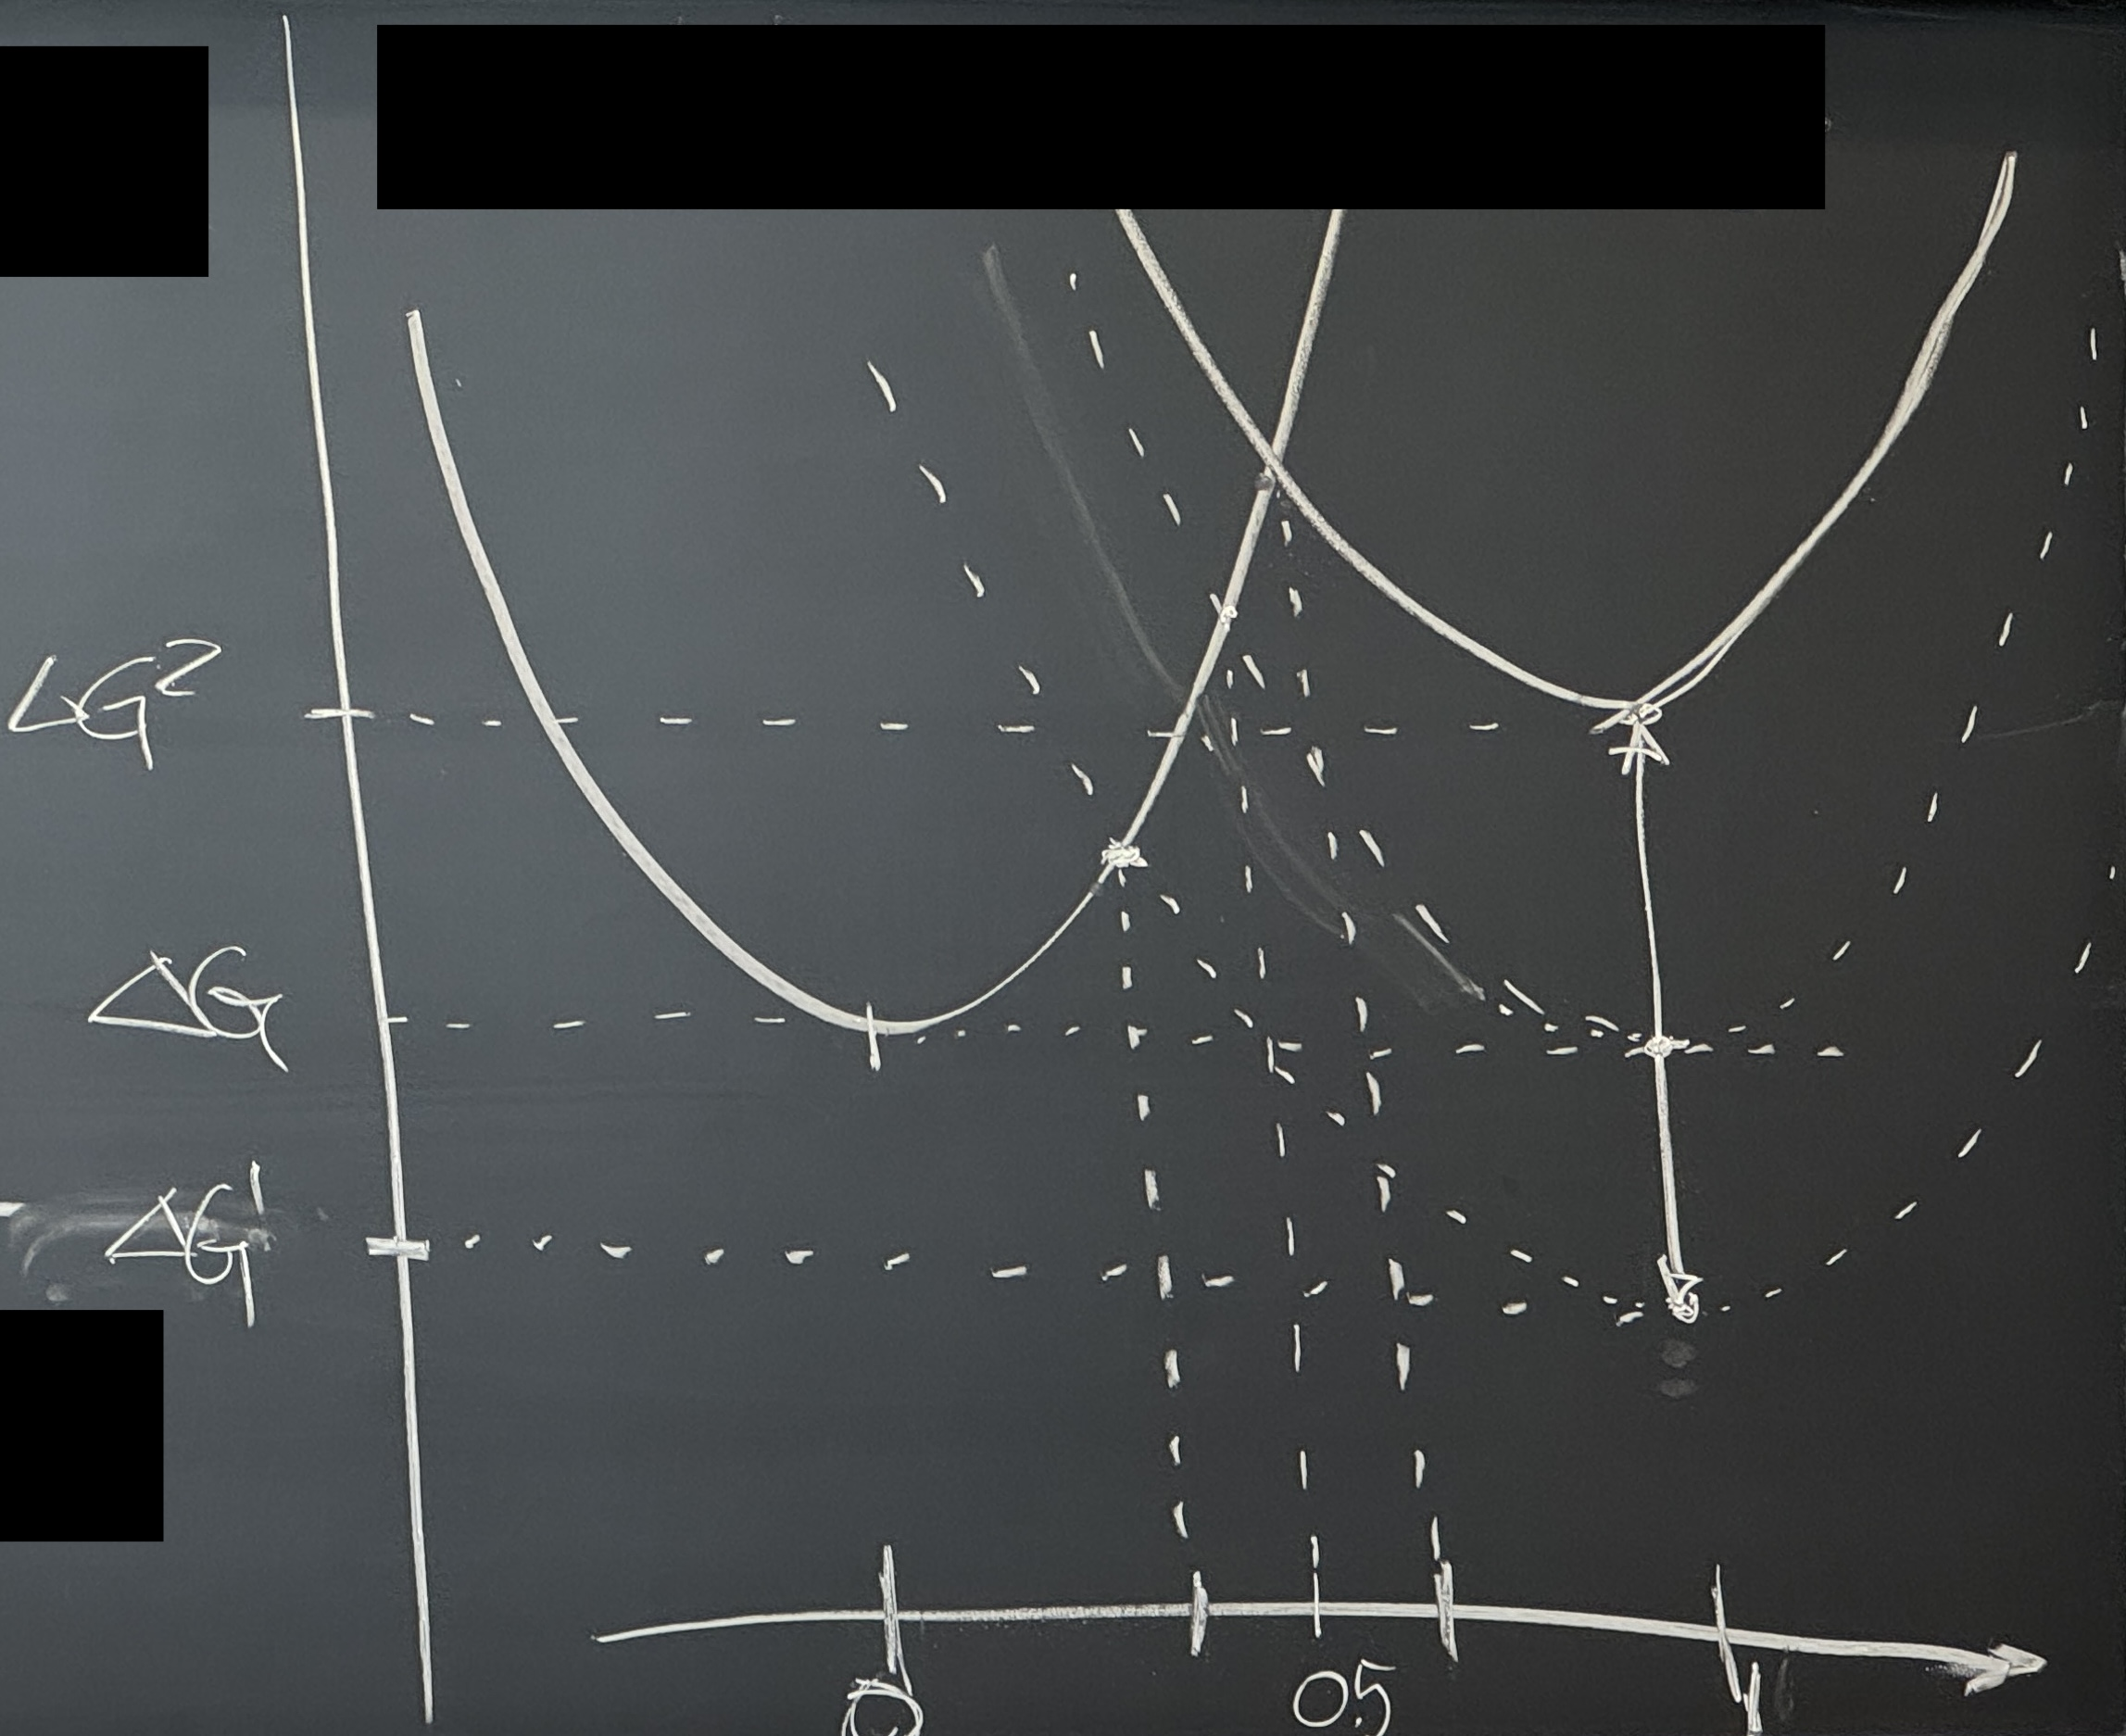
\includegraphics[width=0.4\linewidth]{BEPparabola.JPG}
        \caption{Bell-Evans-Polanyi principle: Parabolic curve crossing.}
        \label{fig:BEPparabola}
    \end{figure}
    \begin{itemize}
        \item Both parabolas should have the same curvature.
        \item Suppose first that the second vertex is lower in energy by $\Delta G^1$.
        \begin{itemize}
            \item This implies that the TST happens at less than 0.5 along the reacton coordinate.
            \item Implication: Exergonic reactions have TSTs lower in energy than the degenerate reaction, and with a TST more like the SMs ("earlier").
        \end{itemize}
        \item If $\Delta G^2>0$, endergonic reactions have a TST more like the products ("later") and higher energy.
        \item This is all collectively known in the literature as the \textbf{Bell-Evans-Polanyi principle}, or alternatively as the \textbf{Hammond postulate}.
    \end{itemize}
    \item Example: Radical halogenation of alkanes.\footnote{See Figure \ref{fig:Hammond} for where Masha covered this.}
    \begin{table}[H]
        \centering
        \small
        \renewcommand{\arraystretch}{1.2}
        \begin{tabular}{c|ccc}
             & \textbf{$\bm{1^\circ}$ \ce{C-H}} & \textbf{$\bm{2^\circ}$ \ce{C-H}} & \textbf{$\bm{3^\circ}$ \ce{C-H}}\\
            \hline
            \ce{F*}  & $1$ & $1.2$ & $1.4$\\
            \ce{Cl*} & $1$ & $3.9$ & $5$\\
            \ce{Br*} & $1$ & $82$  & $1600$\\
        \end{tabular}
        \caption{Relative reactivity rates in radical halogenation.}
        \label{tab:reactRadHalo}
    \end{table}
    \begin{itemize}
        \item Consider the reaction of \ce{F*}, \ce{Cl*}, and \ce{Br*} with primary, secondary, and tertiary \ce{C-H} bonds.
        \item Specifically, consider the relative rate $\krel$ of these reactions.
        \item Selectivity indicates that we should radically halogenate the tertiary \ce{C-H} first.
        \item Additionally, we observe drastically improved selectivity as we get to heavier halogens. Here's a quantitative explanation for this phenomenon.
        \begin{itemize}
            \item The reactants are at about \kcal{100} because that's the approximate \ce{R-H} bond enthalpy; see Masha's list!!
            \item Then \ce{Cl-H} is $\approx\kcal{103}$.
            \item For comparison, the \ce{H-Br} bond dissociation energy is $\approx\kcal{87}$.
        \end{itemize}
        \item Alex now esentially redraws Figure \ref{fig:Hammond}.
    \end{itemize}
    \item This concludes Lecture 16.
    \item We now begin Lecture 17: Isotope effects.
    \item Recall from your previous coursework in quantum mechanics that atomic-scale oscillators have quantized --- not classically continuous --- energies.
    \begin{figure}[h!]
        \centering
        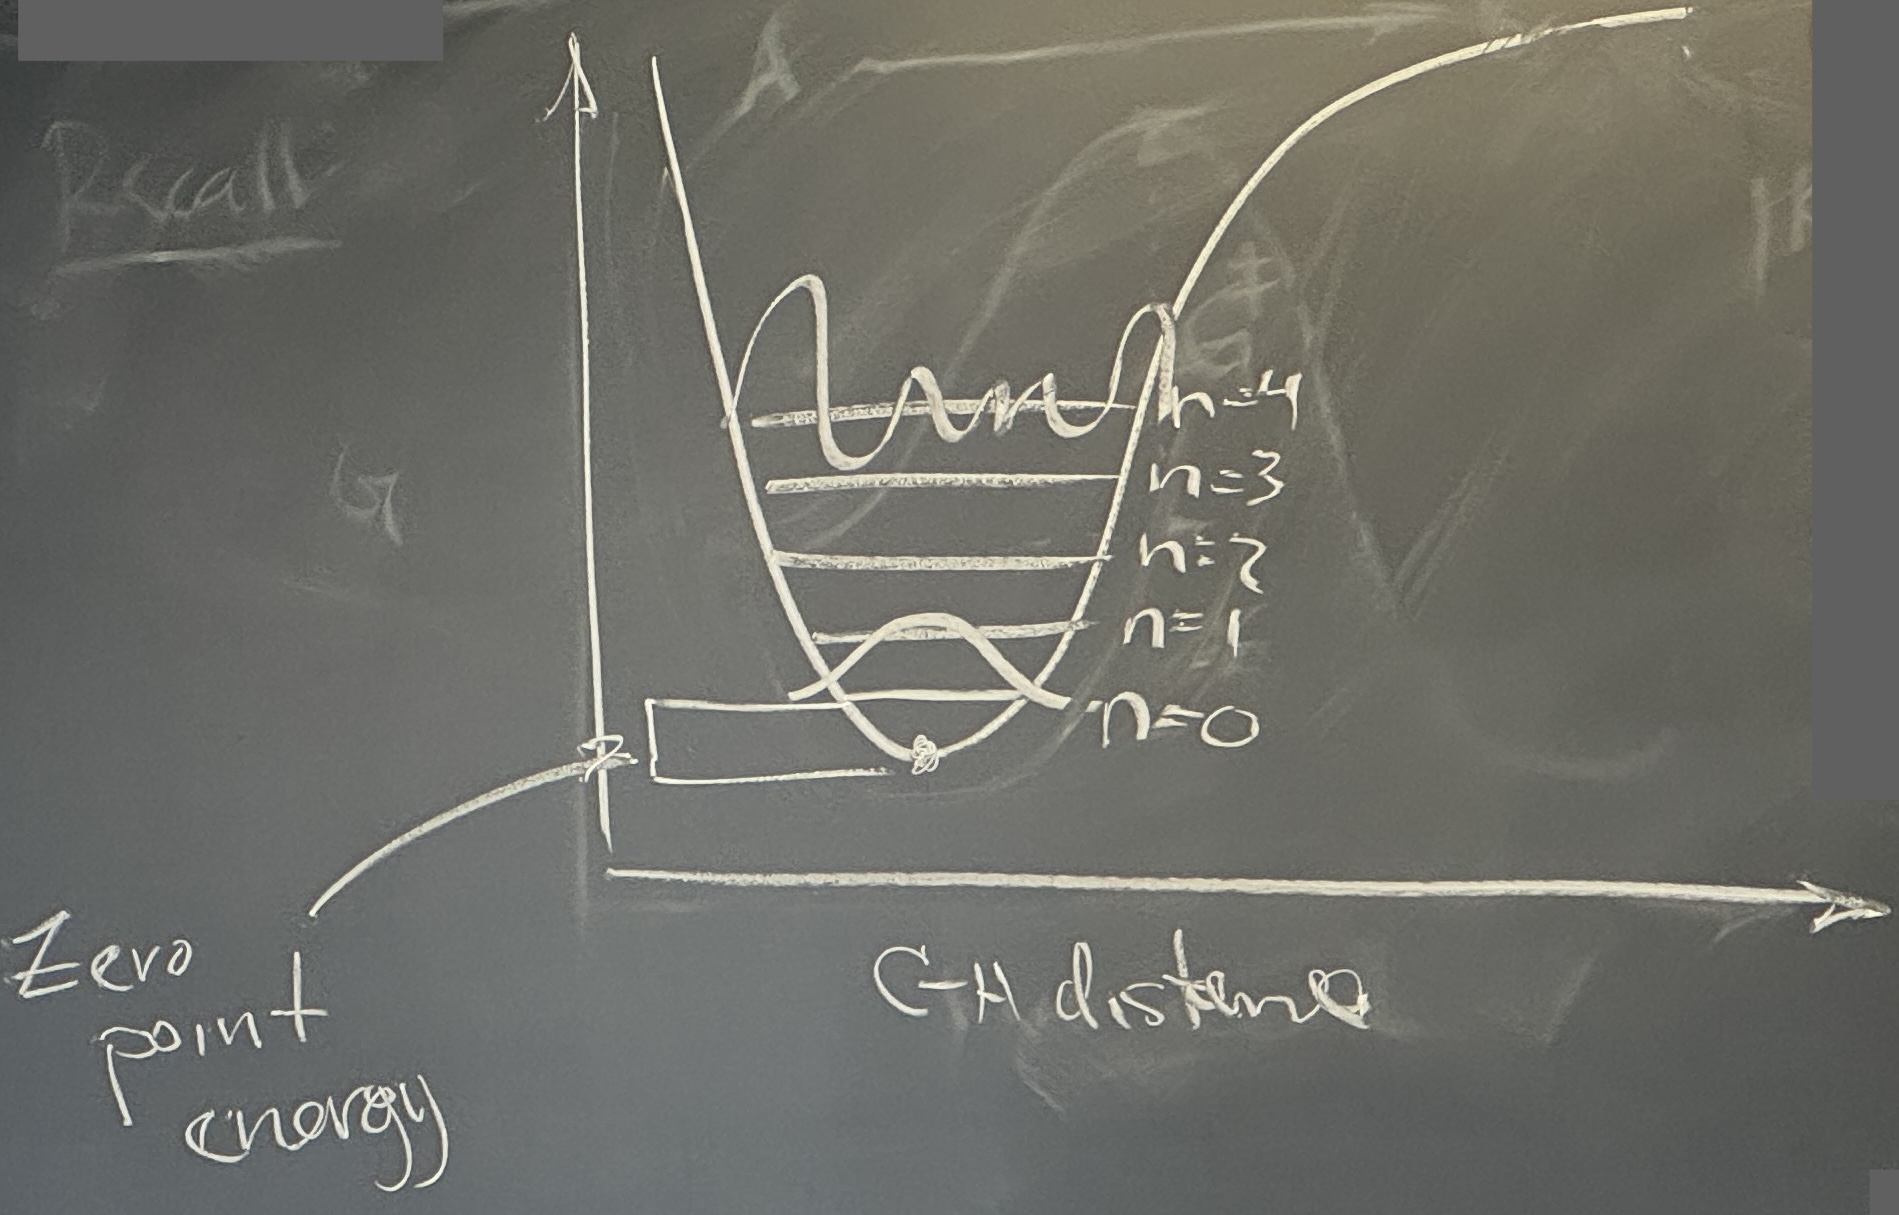
\includegraphics[width=0.5\linewidth]{quantumOsc.JPG}
        \caption{Quantum oscillator potential.}
        \label{fig:quantumOsc}
    \end{figure}
    \begin{itemize}
        \item So while we do have a minimum on the potential energy surface, the molecule does not hang out there because this would require that the quantum particle is static (so we'd know its position and momentum, violating Heisenberg uncertainty).
        \item So at the energy minimum, there is residual energy latent in the system called \textbf{zero-point energy}.
        \item So even in the lowest wave function, there's gonna be some spread of the nuclear position beyond the potential well.
    \end{itemize}
    \item \textbf{Zero-point energy}. \emph{Also known as} \textbf{ZPE}, $\bm{E_0}$.
    \item Quantized vibrational energies.
    \begin{table}[h!]
        \centering
        \small
        \renewcommand{\arraystretch}{1.2}
        \begin{tabular}{cc}
            \textbf{Bond} & $\bm{\mu}$\\
            \hline
            \ce{C-H}           & $0.92$\\
            \ce{C-D}           & $1.72$\\
            \ce{{}^12C-{}^12C} & $6.00$\\
            \ce{{}^12C-{}^13C} & $6.24$\\
        \end{tabular}
        \caption{The reduced mass of common chemical bonds.}
        \label{tab:redMassBond}
    \end{table}
    \begin{itemize}
        \item We have that
        \begin{equation*}
            E_n = h\nu\left( n+\frac{1}{2} \right)
        \end{equation*}
        \item Recall that an (asymmetric) molecule has $3N-6$ vibrational modes.
        \item This frequency of oscillation (per Hooke's law) is related to the force constant and \textbf{reduced mass}.
        \begin{equation*}
            \nu = \frac{1}{2\pi}\sqrt{\frac{k}{\mu}}
        \end{equation*}
        \item Atoms are defined by the number of protons, but we can change the number of neutrons as much as we want! This will change the reduced mass.
        \item The magnitude of isotope effects is the greatest when the reduced mass changes the most.
    \end{itemize}
    \item \textbf{Reduced mass}: The quantity given as follows, where $m_1,m_2$ are the masses of two particles in a system. \emph{Denoted by} $\bm{\mu}$. \emph{Given by}
    \begin{equation*}
        \mu = \frac{m_1m_2}{m_1+m_2}
    \end{equation*}
    \item Looking at the deuterium isotopologue vs. carbon.
    \begin{figure}[h!]
        \centering
        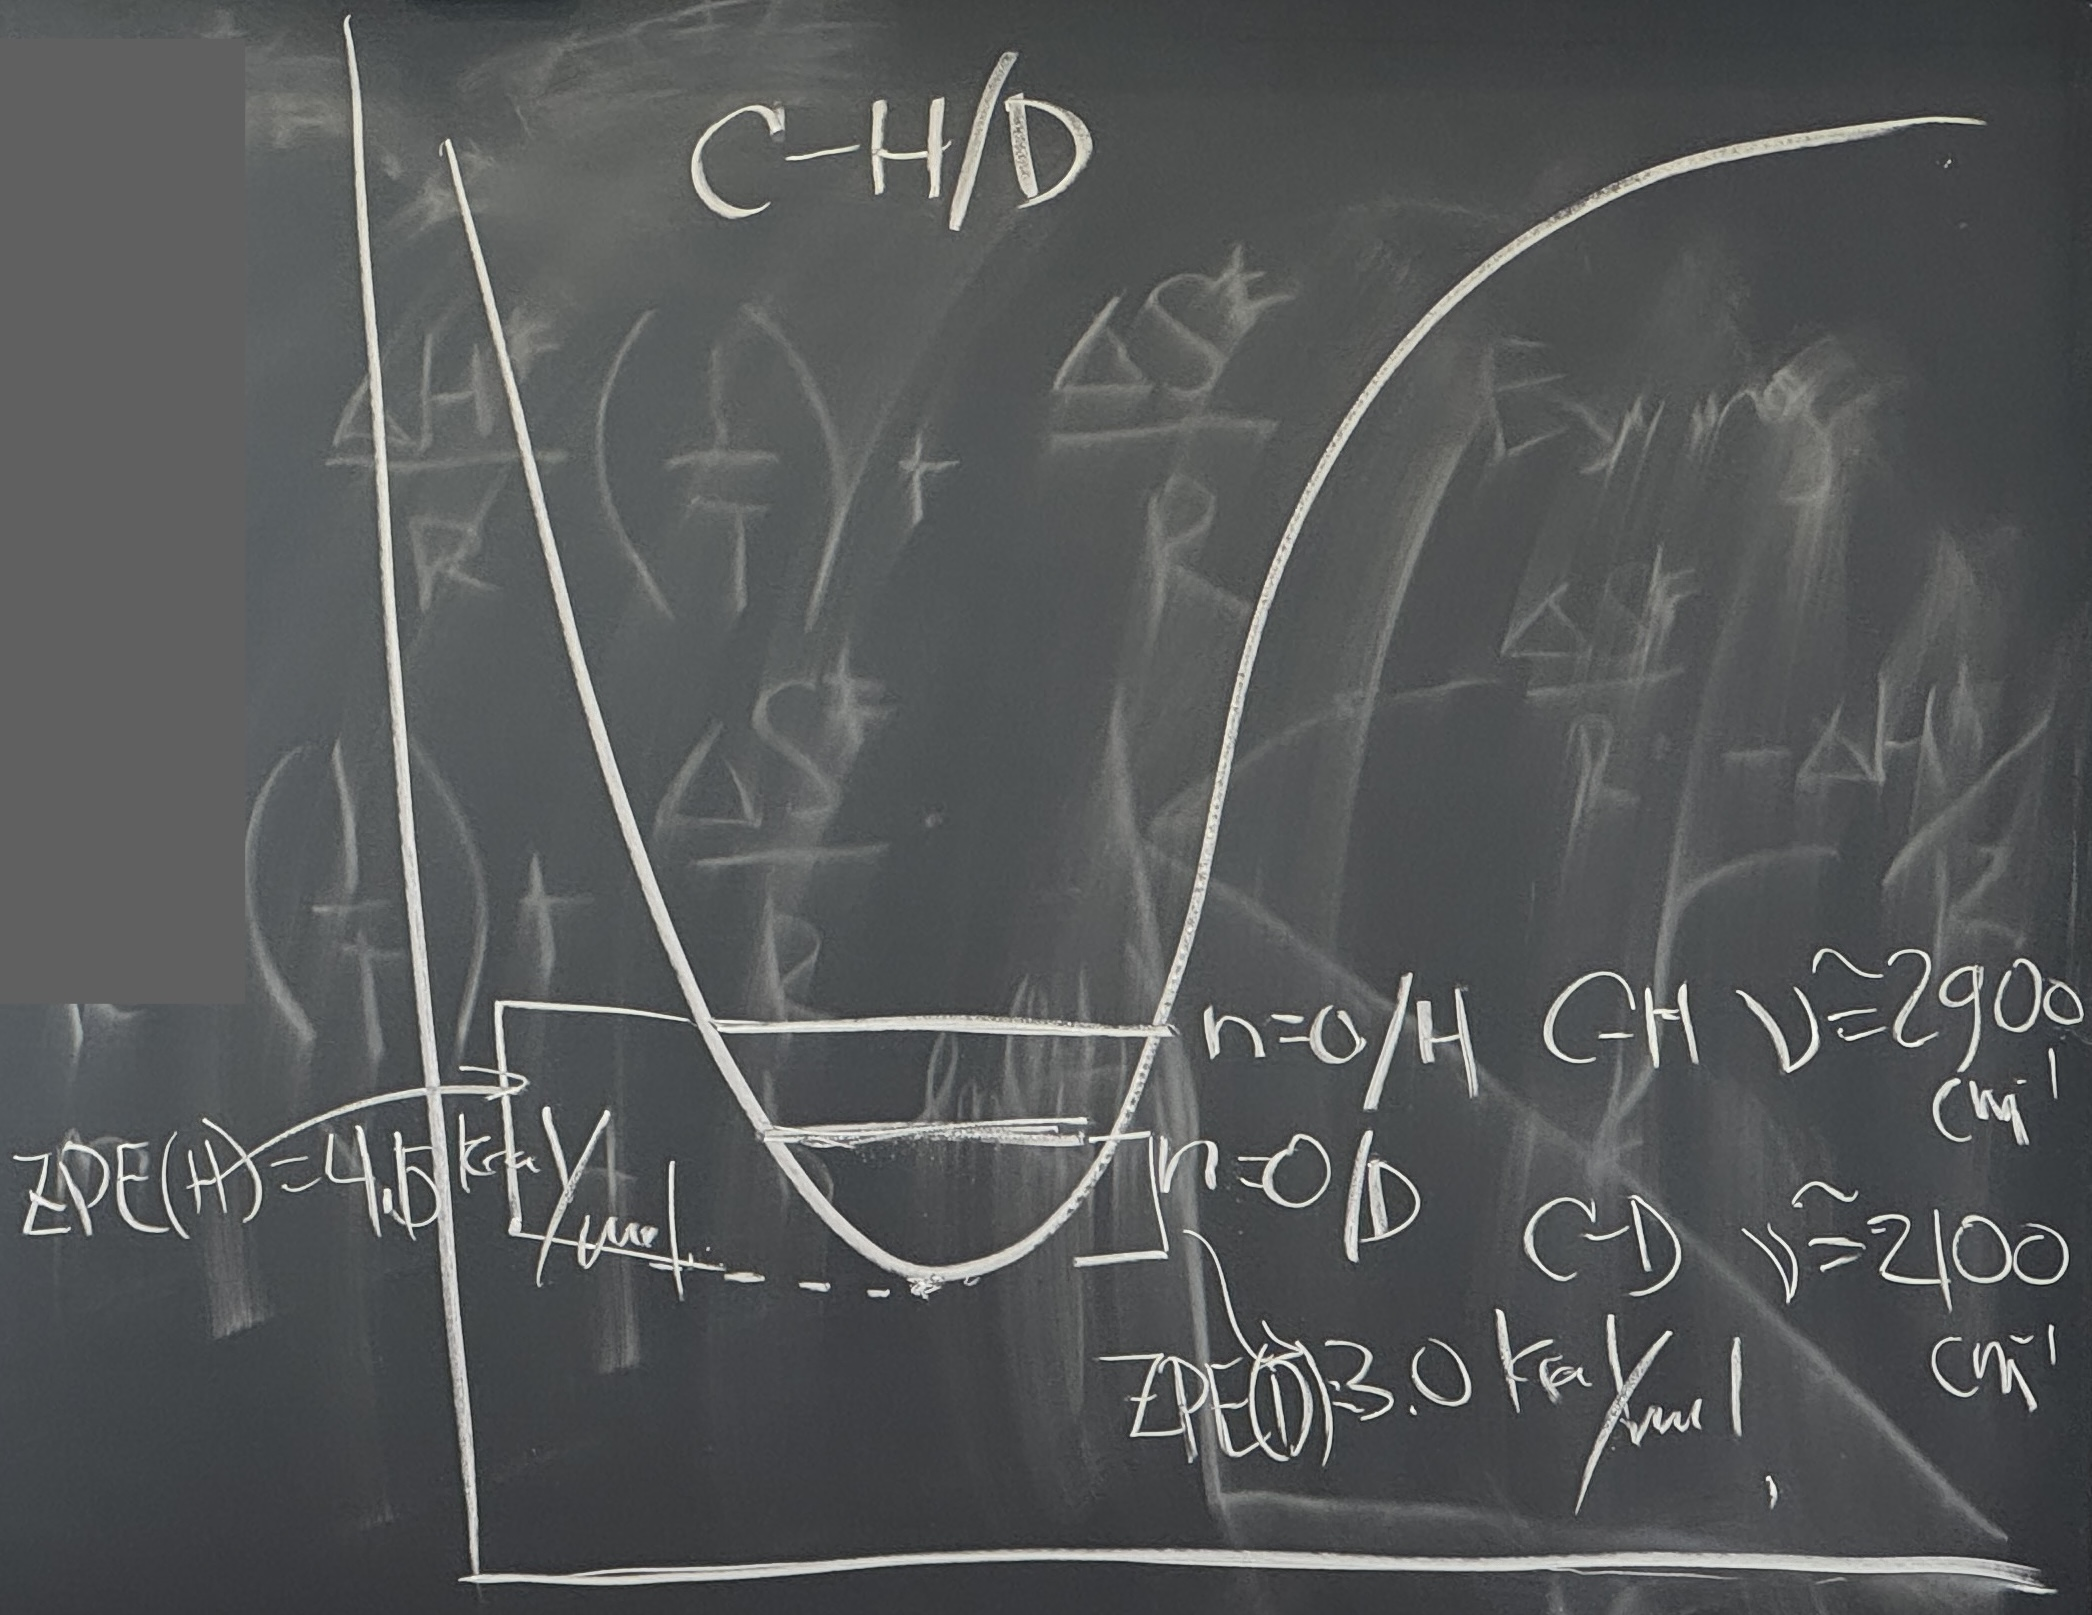
\includegraphics[width=0.45\linewidth]{quantumIso.JPG}
        \caption{Isotopic differences alter the thermodynamic stability of a chemical bond.}
        \label{fig:quantumIso}
    \end{figure}
    \begin{itemize}
        \item The zero-point energy for the \ce{C-D} oscillator is less than for the \ce{C-H} operator.
        \item Thus, \ce{C-H} has $\nu\approx\SI{2900}{\per\centi\meter}$ and \ce{C-D} has $\nu\approx\SI{2100}{\per\centi\meter}$.
        \item This means that it will cost more energy to dissociate a \ce{C-D} bond vs. a \ce{C-H} bond.
        \item The potential is defined only by positive and negative charges, so \emph{it's} the same; it's only the isotopes within it that change.
        \item The zero-point energy of a \ce{C-H} bond is \kcal{4.5}, and the zero-point energy of a \ce{C-D} bond is \kcal{3.0}.
        \item These \kcal{1.5} impact the kinetics reactivity by about sevenfold!
    \end{itemize}
    \pagebreak
    \item Equilibrium isotope effects.
    \begin{figure}[h!]
        \centering
        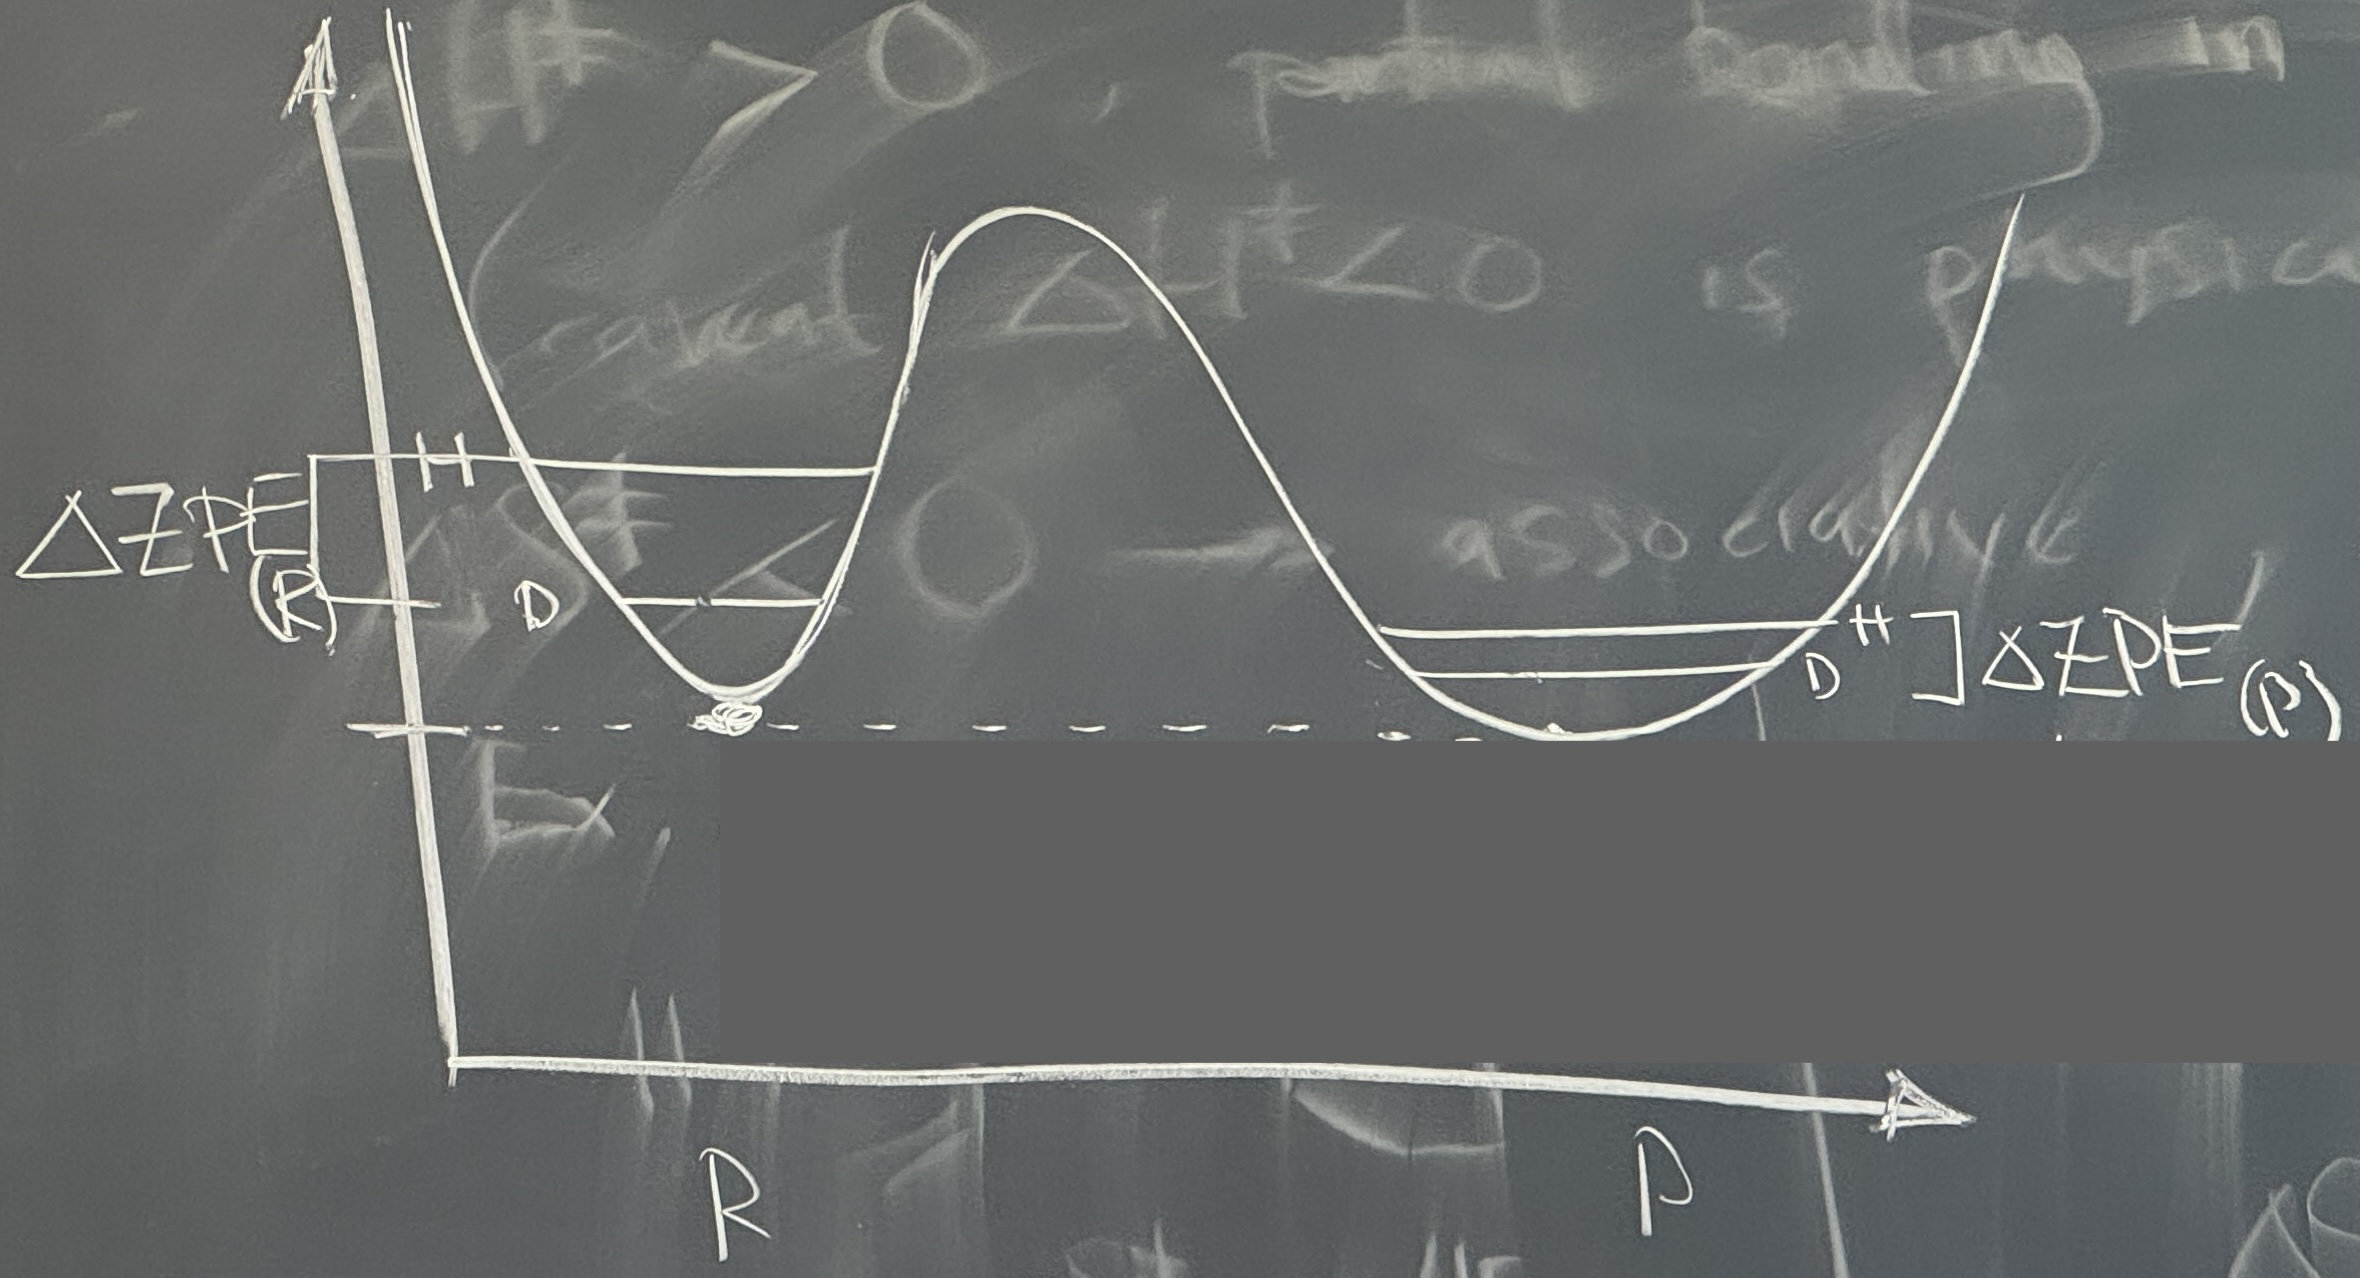
\includegraphics[width=0.55\linewidth]{isotopeEq.JPG}
        \caption{Equilibrium isotope effects.}
        \label{fig:isotopeEq}
    \end{figure}
    \begin{itemize}
        \item Consider an energetically degenerate reaction.
        \item Suppose that the difference in ZPEs is smaller in the products' slack potential.
        \begin{itemize}
            \item Symbolically, $\Delta\ZPE_\text{(R)}>\Delta\ZPE_\text{(P)}$.
        \end{itemize}
        \item So the effective $\Delta G$ for \ce{H} is greater than the one for \ce{D}: $-\Delta G_{\ce{H}}>-\Delta G_{\ce{D}}$.
        \begin{itemize}
            \item Thus, $k_{\ce{H}}/k_{\ce{D}}>1$.
        \end{itemize}
    \end{itemize}
    \item Example: Equilibrium isotope effects during reductive elimination/oxidative addition at transition metals.
    \begin{figure}[h!]
        \centering
        \footnotesize
        \schemestart
            \chemfig{L_nM@{}{}^{n+2}(-[1,,2]CH_3)(-[7,,2]H/D)}
            \arrow{<=>}
            \chemfig{L_nM}
            \arrow{0}[,0.1]\+{,,-1.2em}
            \chemfig{CH_3-[6]H@{}/D}
        \schemestop
        \caption{Reductive elimination of methane.}
        \label{fig:redElimCH4}
    \end{figure}
    \begin{itemize}
        \item Consider a generic metal-ligand complex (\ce{L_nM}) undergoing the reaction in Figure \ref{fig:redElimCH4}.
        \item The typical BDE for a \ce{M-H} bond is \kcalr{40}{80}.
        \begin{itemize}
            \item The BDE for a methane \ce{H_3C-H} bond is \kcal{104}.
        \end{itemize}
        \item Since the metal potential is shallower, it is slacker and hence has a lower associated force constant.
        \begin{itemize}
            \item Symbolically, $k_{\ce{M-H}}<k_{\ce{C-H}}$.
        \end{itemize}
        \item Since the ZPE difference is smaller in the more slack potential (per Figure \ref{fig:isotopeEq}), it follows that
        \begin{equation*}
            \Delta\ZPE_{\ce{M-H/D}} < \Delta\ZPE_{\ce{C-H/D}}
        \end{equation*}
        \item Takehome: Deuterated species prefer to be in the well with the stronger force constant.
    \end{itemize}
    \item Accounting for the anharmonicity\footnote{How is this related to anharmonicity??} in the potential wells.
    \begin{figure}[H]
        \centering
        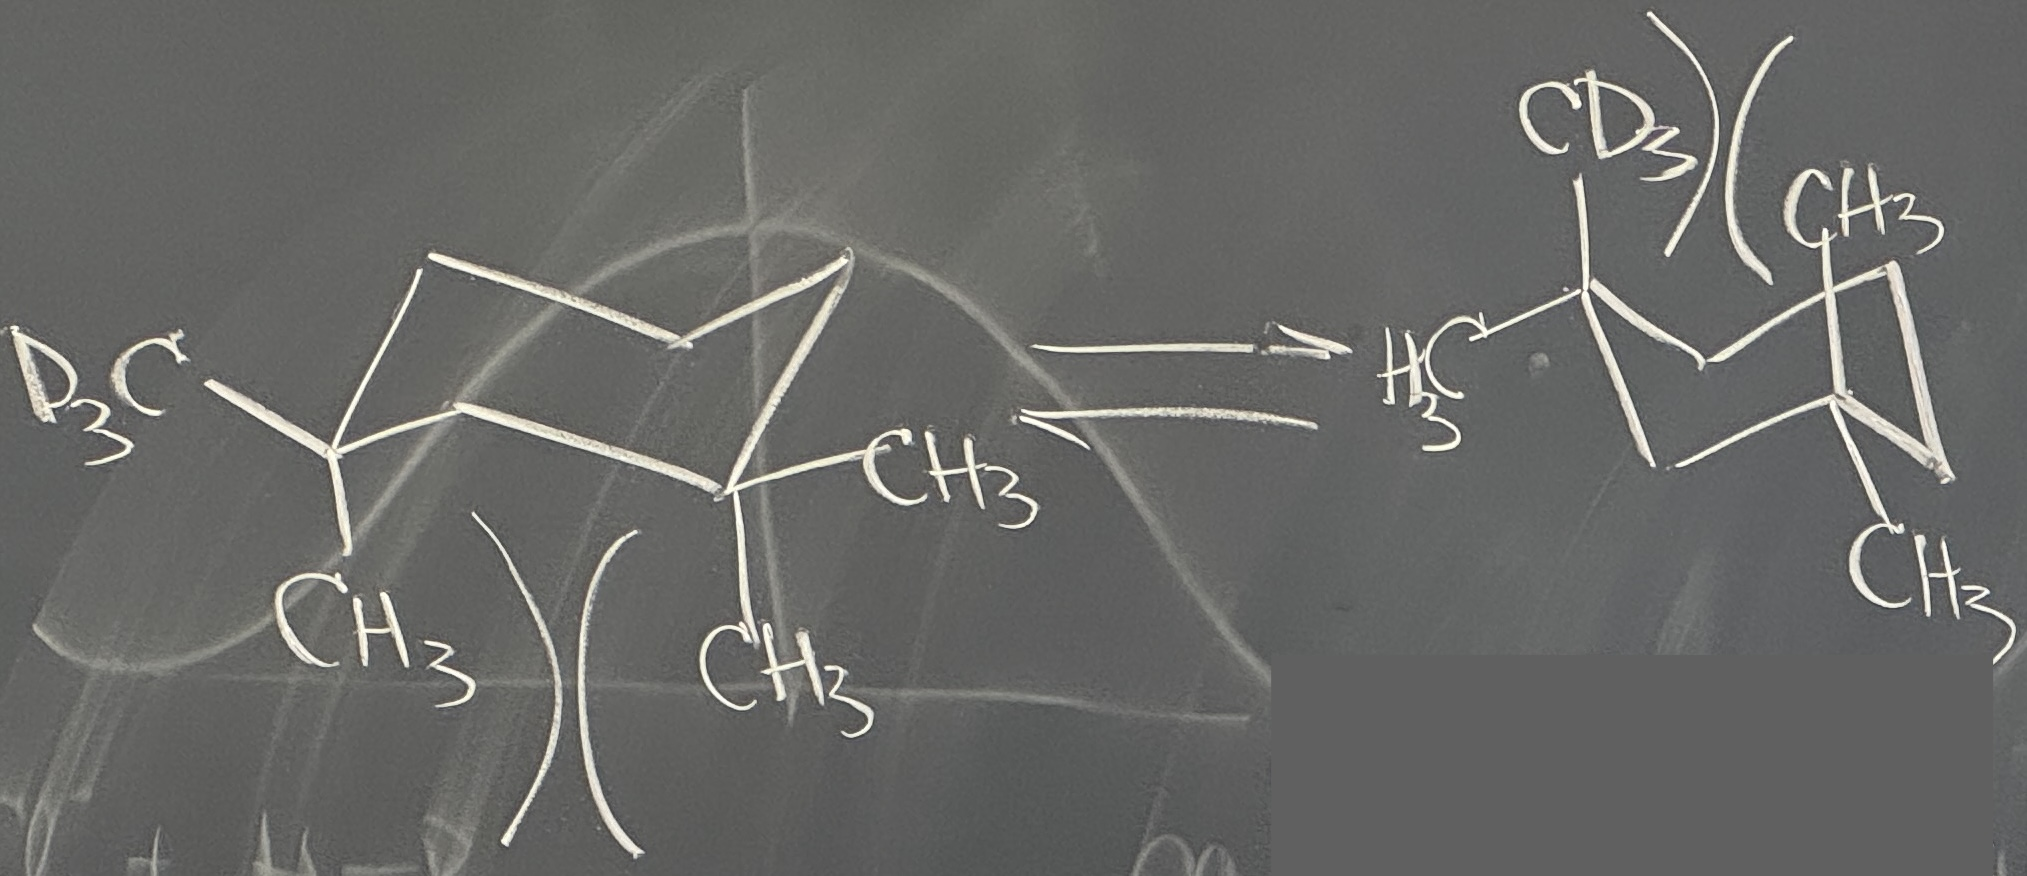
\includegraphics[width=0.35\linewidth]{isotopeSteric.JPG}
        \caption{Steric isotope effects.}
        \label{fig:isotopeSteric}
    \end{figure}
    \begin{itemize}
        \item Consider the ring flip of 1,1,3,3-tetramethylcyclohexane, with one of the methyl groups actually a \ce{CD3} group.
        \item Experimentally, we observe that
        \begin{equation*}
            K = \frac{\cnc{CD3 ax}}{\cnc{CD3 eq}} = 1.042
        \end{equation*}
        at $-\SI{100}{\celsius}$.
        \item It is preferable to have the \ce{CD3} group axial because it is smaller: The lower vibrational amplitude $\nu$ for \ce{C-D} bonds relative to \ce{C-H} bonds literally shrinks the sterics of the group \parencite[430,434]{bib:Anslyn}.
    \end{itemize}
    \item How can we link equilibrium isotope effects to kinetics?
    \begin{itemize}
        \item Like at the beginning of class, we use transition state theory!
        \item Indeed, let's apply our understanding of equilibrium isotope effects to the quasi-equilibrium between the starting materials and transition state. This can give us valuable insight into the relative rates of reaction for heavier vs. lighter isotopologues.
    \end{itemize}
    \item Kinetic isotope effects.
    \begin{figure}[h!]
        \centering
        \begin{tikzpicture}[
            every node/.style=black
        ]
            \small
            \draw [stealth-stealth] (0,4) -- (0,0) -- (7,0);
            \node [below] at (1.5,0) {\ce{C-H + *X}};
            \node [below] at (4,0) {$[\ce{C***H***X}]^\ddagger$};
            \node [below] at (6.5,0) {\ce{C* + H-X}};
    
            \footnotesize
            \draw [grx,thick,name path=PES] (0.3,3.8)
                to[out=-85,in=180,in looseness=0.7] (1.5,0.8)
                to[out=0,in=180,out looseness=0.7] (4,3.2)
                to[out=0,in=180,in looseness=0.6] (6.5,0.1)
                to[out=0,in=-150,out looseness=0.6] (6.8,0.2)
            ;
    
            \footnotesize
            \path [name path=CH] (0.5,1.3) -- ++(2,0);
            \draw [grx,name intersections={of=PES and CH}] (intersection-1) node[left]{\ce{C-H}} -- (intersection-2);
            \path [name path=CD] (0.5,1.0) -- ++(2,0);
            \draw [grx,name intersections={of=PES and CD}] (intersection-1) node[left]{\ce{C-D}} -- (intersection-2);
            \draw [|-|] (2.4,1) -- node[right]{$\Delta\ZPE_\text{(GS)}^{\textcolor{white}{(GS)}}$} ++(0,0.3);
    
            \filldraw [grx,thick,name path=PESo1] (4,3.2) to[out=180,in=-30] (2.5,3.57) -- (2.5,3.63) to[out=-30,in=180] cycle;
            \draw [grx,thick,dashed,name path=PESo2] (4,3.2) to[out=0,in=-150] (5.5,3.6);
            \path [name path=CH] (2.5,3.4) -- ++(3,0);
            \draw [grx,name intersections={of=PESo1 and CH},name intersections={of=PESo2 and CH}] (intersection-2) node[above left=-2pt,xshift=-5mm]{\ce{C-H}} -- (intersection-1);
            \path [name path=CD] (2.5,3.3) -- ++(3,0);
            \draw [grx,name intersections={of=PESo1 and CD},name intersections={of=PESo2 and CD}] (intersection-2) node[below left=-2pt]{\ce{C-D}} -- (intersection-1);
            \draw [|-|] (5.5,3.3) -- node[right]{$\Delta\ZPE_\text{(TS)}^{\textcolor{white}{(TS)}}$} ++(0,0.1);
        \end{tikzpicture}
        \caption{Kinetic isotope effects.}
        \label{fig:KIE}
    \end{figure}
    \begin{itemize}
        \item Consider the HAT reaction
        \begin{equation*}
            \ce{C-H + *X -> C* + H-X}
        \end{equation*}
        \begin{itemize}
            \item This is a nondegenerate reaction, energetically.
        \end{itemize}
        \item Recall that transition structures are maxima along one direction, but minima along every other direction in the hyperspace (see Figure \ref{fig:EDtBuClcon}).
        \begin{itemize}
            \item It follows that $\Delta\ZPE$ is relatively small in the TS, because TS potentials are pretty slack compared with bond potentials.
        \end{itemize}
        \item The important equation we can write from the above diagram is
        \begin{equation*}
            \Delta\Delta G^\ddagger = \Delta\Delta\ZPE
            = \Delta\ZPE_\text{(GS)}-\Delta\ZPE_\text{(TS)}
        \end{equation*}
        \begin{itemize}
            \item This means that it's easier to take \ce{C-H} to the transition state than \ce{C-D}.
            \item This is a \textbf{normal KIE}, where $k_{\ce{H}}/k_{\ce{D}}>1$.
            \item This is also primary ($1^\circ$) because the isotope-sensitive bond is the one being broken/made.
        \end{itemize}
    \end{itemize}
    \item \textbf{Inverse KIEs} involve cases in which $k_{\ce{D}}/k_{\ce{H}}<1$.
    \begin{itemize}
        \item This is also $1^\circ$.
    \end{itemize}
    \item We can also have \textbf{secondary} KIEs, where we label a position potentially far from the reactive site.
    \item Next time: Using KIEs to diagnose reaction mechanisms, single isotopologues under different reaction conditions give us different information, etc. Takeaways: KIEs are super useful.
\end{itemize}



\section{Kinetic Isotope Effects}
\begin{itemize}
    \item \marginnote{11/7:}Lecture 17 recap.
    \begin{itemize}
        \item Potential energy surfaces remain unperturbed when switching between isotopologues because the potentials are defined by the electrostatic charge densities of the relevant nuclei.
        \begin{itemize}
            \item However, the energetic position within the well of the vibrational wave functions varies with the reduced mass.
        \end{itemize}
        \item \ce{C-H/D} isotope effects lead to six- or sevenfold selectivity differences.
    \end{itemize}
    \item A note on the thermodynamic population of various energy levels.
    \begin{itemize}
        \item Almost all molecules reside at the zero-point energy $E_0$, so only considering $\Delta G$'s and $\Delta G^\ddagger$'s between zero-point energies \emph{is} a good approximation.
    \end{itemize}
    \item Today: Finalizing some of the descriptive aspects of isotope effects, especially in the transition state structure.
    \item Consider an atom-transfer reaction, like in Figure \ref{fig:KIE}.
    \begin{figure}[h!]
        \centering
        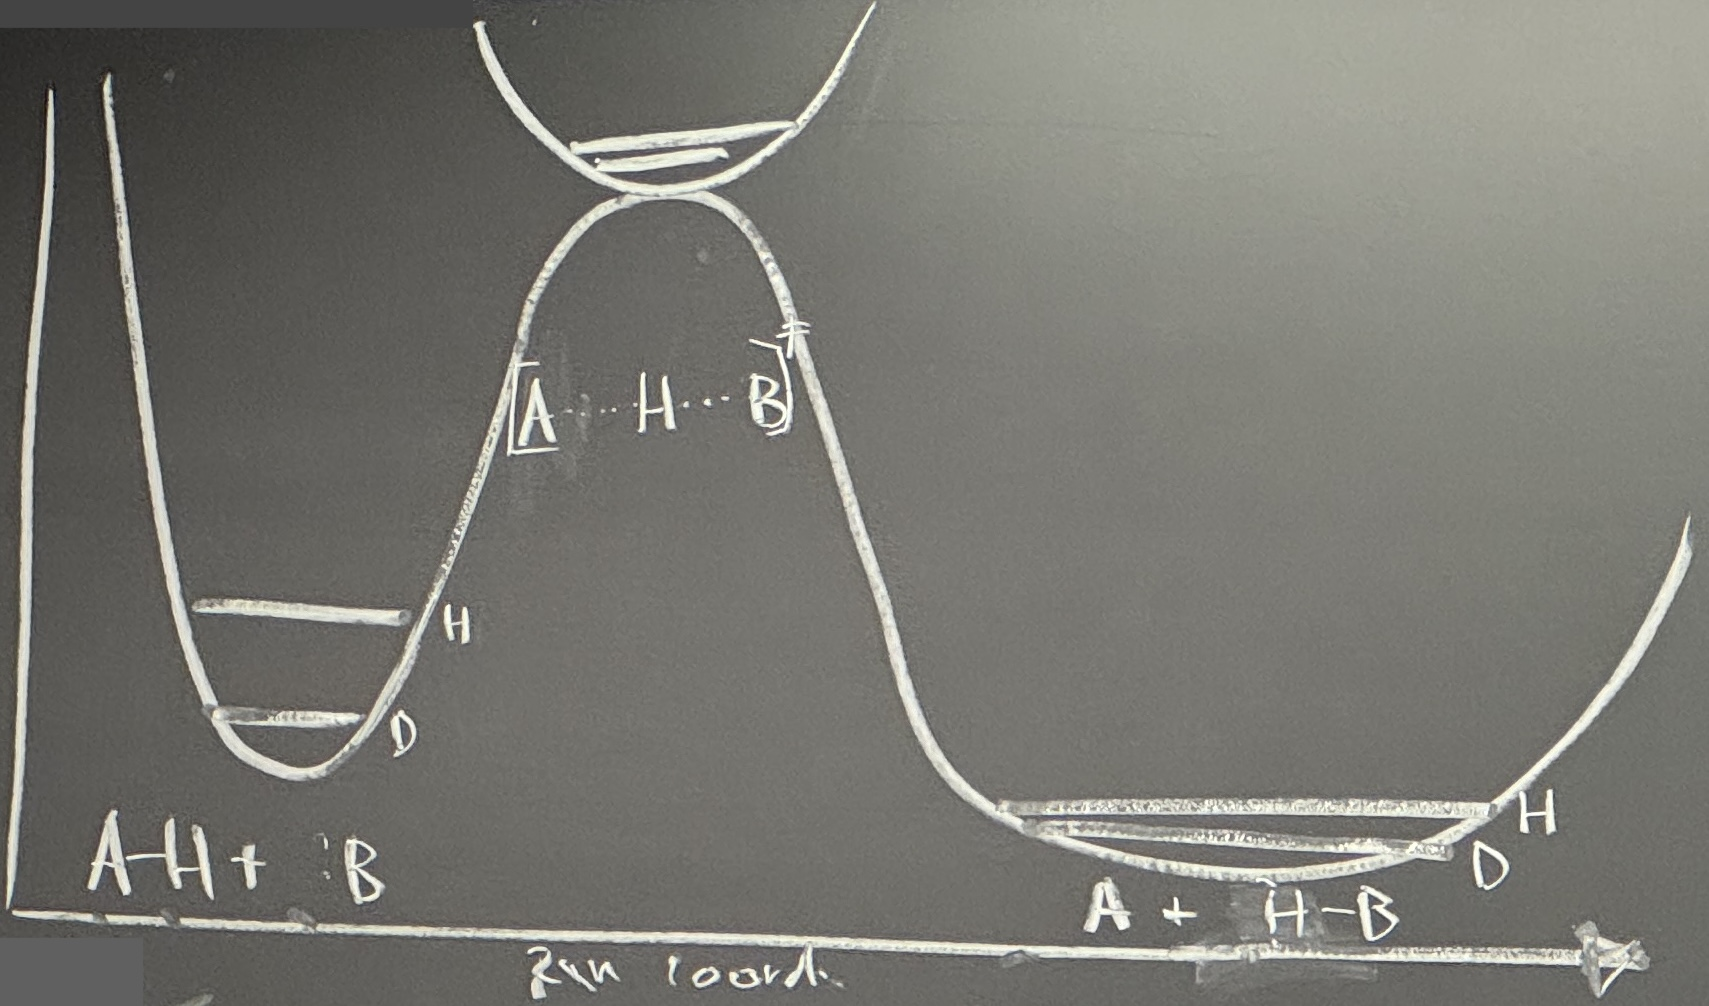
\includegraphics[width=0.45\linewidth]{ATPES.JPG}
        \caption{Atom-transfer potential energy surface.}
        \label{fig:ATPES}
    \end{figure}
    \begin{itemize}
        \item We may think of either an acid-base deprotonation or an HAT; it really doesn't matter.
        \item The ensemble $[\ce{A***H***B}]^\ddagger$ is the transition structure.
        \begin{itemize}
            \item It lives at a saddle point, so all of its vibrational modes live in the orthogonal potentials.
        \end{itemize}
        \item Since the TS is triatomic and linear, it has $3N-5=4$ vibrational modes.
        \begin{itemize}
            \item More specifically, it has 3 different \emph{kinds} of vibrational modes, since the bending mode can happen in two orthogonal directions.
        \end{itemize}
    \end{itemize}
    \item In the parlance of vibrational spectroscopy, the molecular motion in the transition state is the extreme of the \textbf{asymmetric stretch}.
    \begin{figure}[h!]
        \centering
        \begin{subfigure}[b]{0.25\linewidth}
            \centering
            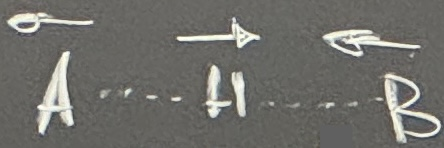
\includegraphics[width=0.5\linewidth]{ATviba.JPG}
            \caption{Asymmetric stretch.}
            \label{fig:ATviba}
        \end{subfigure}
        \begin{subfigure}[b]{0.25\linewidth}
            \centering
            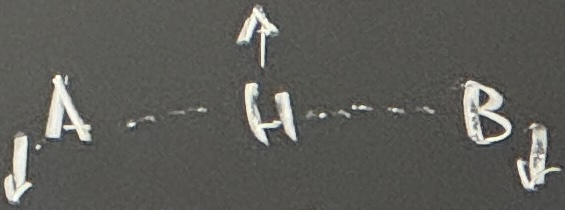
\includegraphics[width=0.6\linewidth]{ATvibb.JPG}
            \caption{Symmetric bend.}
            \label{fig:ATvibb}
        \end{subfigure}
        \begin{subfigure}[b]{0.25\linewidth}
            \centering
            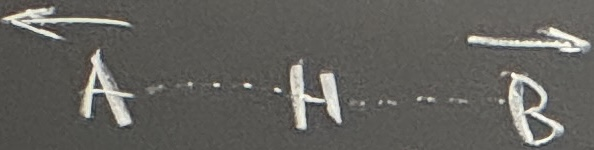
\includegraphics[width=0.65\linewidth]{ATvibc.JPG}
            \caption{Symmetric stretch.}
            \label{fig:ATvibc}
        \end{subfigure}
        \caption{Atom-transfer vibrational modes.}
        \label{fig:ATvib}
    \end{figure}
    \pagebreak
    \begin{itemize}
        \item This asymmetric stretch corresponds to the reaction coordinate.
        \begin{itemize}
            \item This is the vibrational mode along which we're minimizing.
            \item No vibrational value that we assign to this mode.
            \begin{itemize}
                \item Downwards concavity at this point means all frequencies are imaginary.
                \item If you use DFT to compute force constants in the TS (which we always should), it will tell us that the force constants are imaginary.
            \end{itemize}
        \end{itemize}
        \item The other modes include the \textbf{symmetric bending mode}.
        \begin{itemize}
            \item This does modify the KIE. It contributes, but it a minor way that we'll discuss later.
        \end{itemize}
        \item Then there's the \textbf{symmetric stretch}.
        \begin{itemize}
            \item This mode most dramatically affects KIEs; in fact, it is the primary determinant of the KIE because it is the stretch affected when you switch isotopes.
        \end{itemize}
    \end{itemize}
    \item If the \ce{H} or \ce{D} atom is completely stationary in the TS, the isotopic sensitivity of the transition state goes to zero! Here are the conditions under which this happens.
    \begin{figure}[h!]
        \centering
        \begin{tikzpicture}[
            every node/.style=black
        ]
            \small
            \node at (0,4) {$[\ce{A***H/D***B}]^\ddagger$};
    
            \draw [gry,thick,name path=PESo] (-1.5,3.6)
                to[out=-30,in=180] (0,3.2)
                to[out=0,in=-150] (1.5,3.6)
            ;
            \draw [grx,thick,name path=PES] (-3.3,1.5)
                to[out=-70,in=180,in looseness=0.7] (-2.5,0.8)
                to[out=0,in=180,out looseness=0.7] (0,3.2)
                to[out=0,in=180,in looseness=0.7] (2.5,0.8)
                to[out=0,in=-110,out looseness=0.7] (3.3,1.5)
            ;
    
            \path [name path=CH] (-3.5,1.3) -- ++(2,0);
            \draw [grx,name intersections={of=PES and CH}] (intersection-1) -- (intersection-2);
            \path [name path=CD] (-3.5,1.0) -- ++(2,0);
            \draw [grx,name intersections={of=PES and CD}] (intersection-1) -- (intersection-2);
    
            \path [name path=CH] (1.5,1.3) -- ++(2,0);
            % \draw [grx,name intersections={of=PES and CH}] (intersection-1) -- (intersection-2);
            \path [name path=CD] (1.5,1.0) -- ++(2,0);
            % \draw [grx,name intersections={of=PES and CD}] (intersection-1) -- (intersection-2);
    
            \path [name path=C] (-1.5,3.3) -- ++(3,0);
            \draw [gry,name intersections={of=PESo and C}] (intersection-1) -- (intersection-2);
        \end{tikzpicture}
        \caption{Thermoneutral kinetic isotope effects.}
        \label{fig:KIEtherm}
    \end{figure}
    \begin{itemize}
        \item The reaction has to be thermoneutral.
        \item \ce{A} and \ce{B} need to be identical (or at least have the same mass).
        \begin{itemize}
            \item A thermoneutral HAT between atoms of very different masses gives some interesting KIEs.
            \item This would be very devious to put on the exam!!
        \end{itemize}
        \item With zero difference in zero-point energy between \ce{A-H} and \ce{A-D} in the transition state but still a good difference in the starting materials, it follows that $\Delta\Delta G^\ddagger$ should be fairly large.
        \begin{itemize}
            \item Hence the kinetic isotope effect is pretty large in this regime.
        \end{itemize}
    \end{itemize}
    \item What about when the TST is asymmetric?
    \begin{figure}[h!]
        \centering
        \begin{subfigure}[b]{0.4\linewidth}
            \centering
            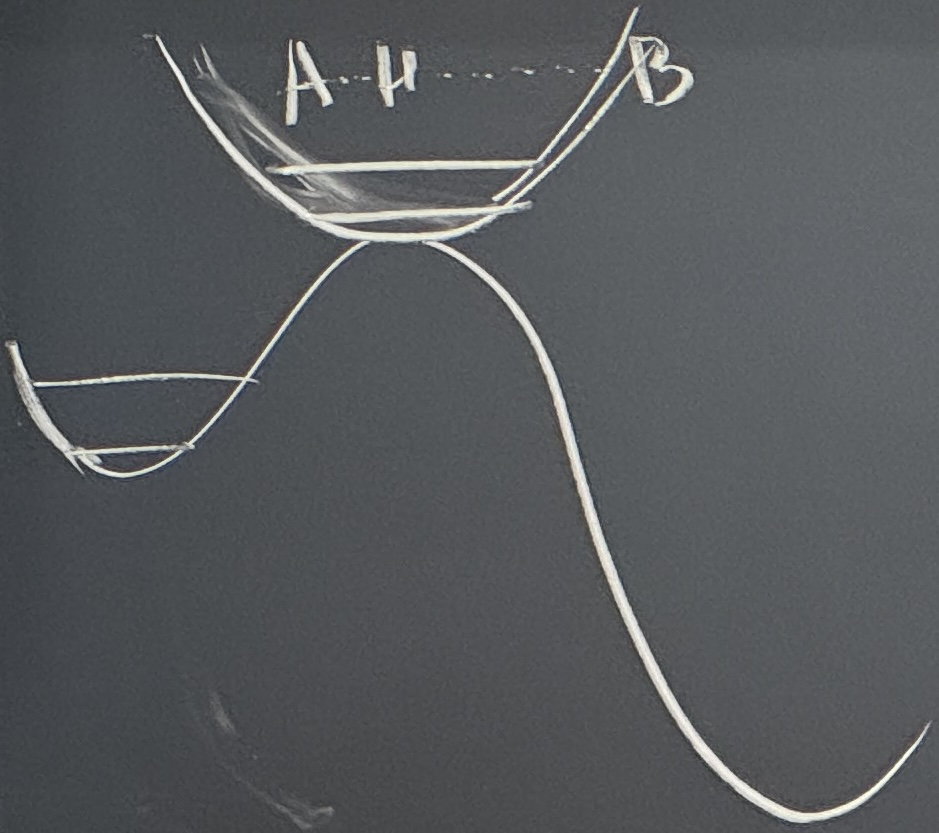
\includegraphics[width=0.8\linewidth]{KIEasya.JPG}
            \caption{Exergonic.}
            \label{fig:KIEasya}
        \end{subfigure}
        \begin{subfigure}[b]{0.4\linewidth}
            \centering
            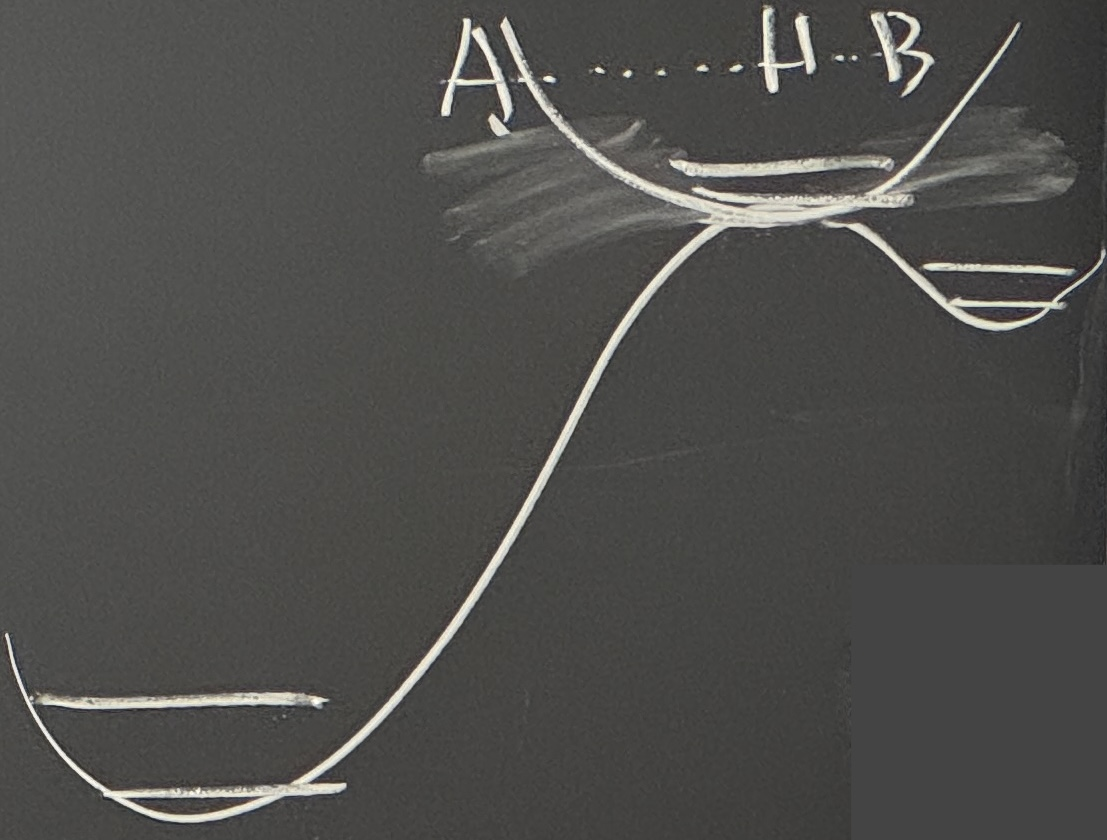
\includegraphics[width=0.8\linewidth]{KIEasyb.JPG}
            \caption{Endergonic.}
            \label{fig:KIEasyb}
        \end{subfigure}
        \caption{Thermodynamically asymmetric kinetic isotope effects.}
        \label{fig:KIEasy}
    \end{figure}
    \begin{itemize}
        \item Consider an exergonic reaction (Figure \ref{fig:KIEasya}).
        \begin{itemize}
            \item Per the Hammond postulate, the transition state will resemble the starting materials.
            \item Thus, the difference in energy $\Delta E$ between the \ce{A-H} and \ce{A-D} transition states should be quite similar to the respective $\Delta E$ in the starting materials.
            \item Hence, $\Delta\Delta G^\ddagger$ smaller, so the KIEs are less than maximal.
        \end{itemize}
        \item Consider an endergonic reaction (Figure \ref{fig:KIEasyb}).
        \begin{itemize}
            \item Per the Hammond postulate, the transition state will resemble the products
            \item Thus, $\Delta E$ will be nonzero (as it is in the products).
            \item Hence, $\Delta\Delta G^\ddagger$ is once again smaller than its thermoneutral maximum, so the KIEs are correspondingly smaller than maximum.
        \end{itemize}
        \item Takeaway: Kinetic isotope effects can give us a window in the precise atomic composition and orientation of the transition structure.
    \end{itemize}
    \item We can measure the extent to which the magnitude of a kinetic isotope effect varies with thermodynamic asymmetry.
    \begin{figure}[h!]
        \centering
        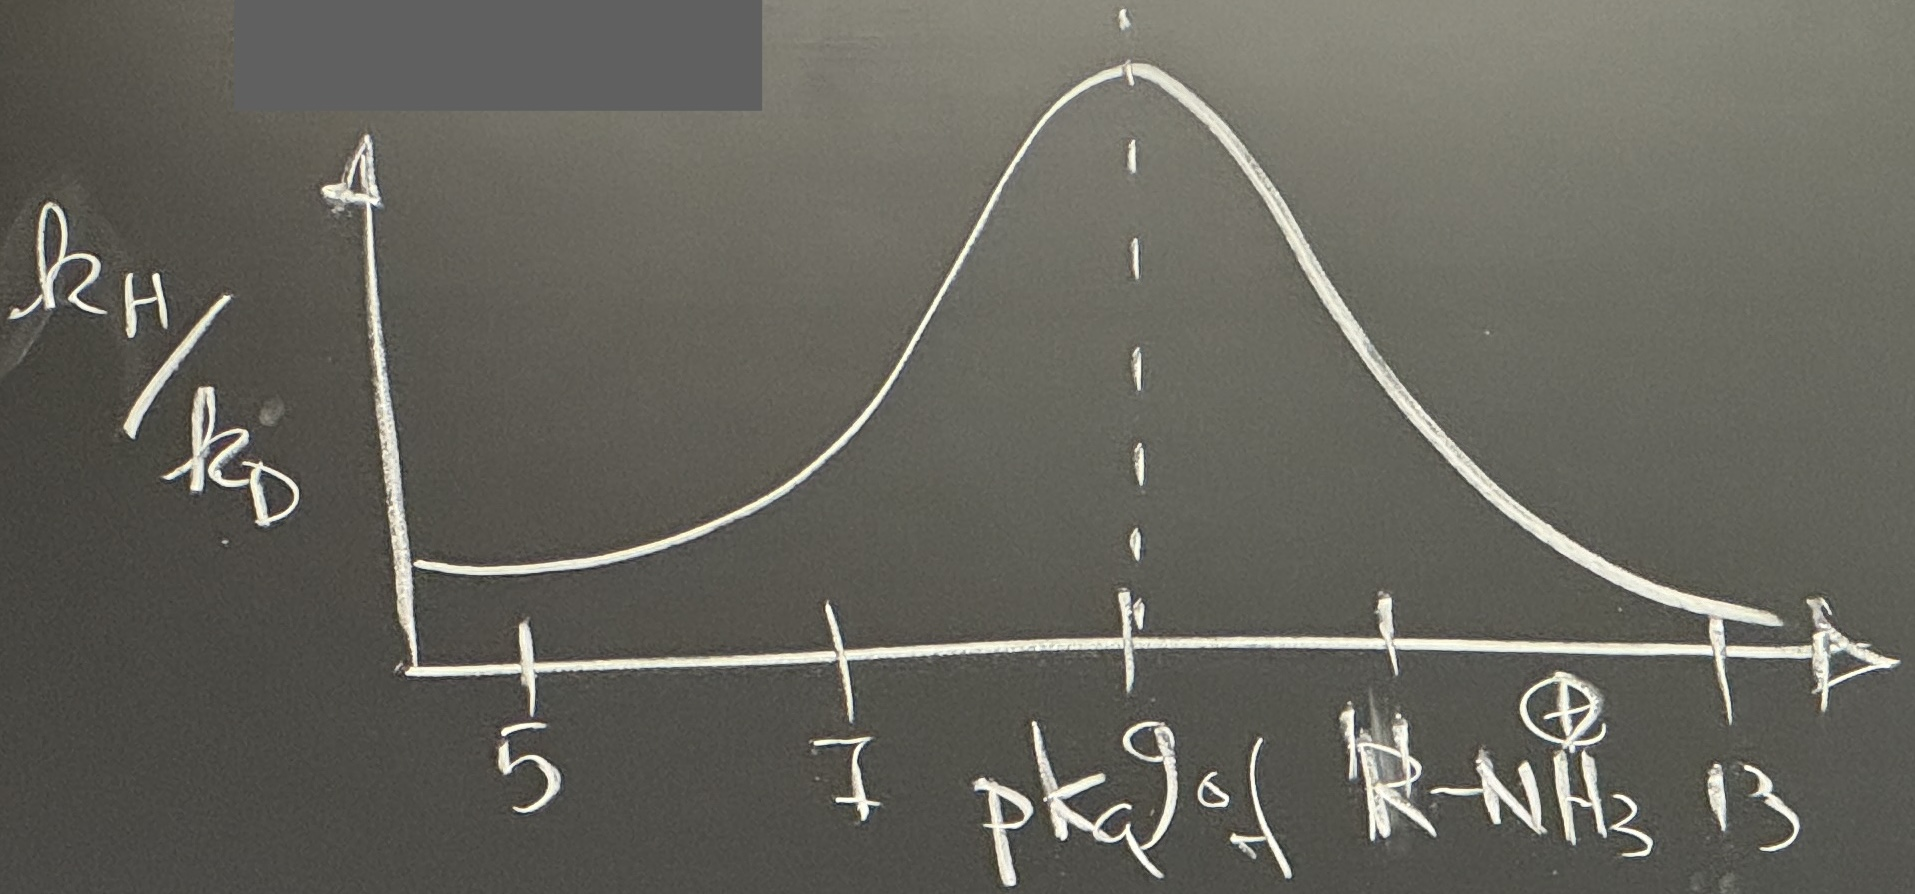
\includegraphics[width=0.4\linewidth]{KIEasyVary.JPG}
        \caption{Variation in kinetic isotope effects with thermodynamic asymmetry.}
        \label{fig:KIEasyVary}
    \end{figure}
    \begin{itemize}
        \item Consider the following acid-base deprotonation.
        \begin{center}
            \footnotesize
            \schemestart
                \chemfig{Me-[:30](-[:110]D/H)(-[:70]H@{}/D)-[:-30]NO_2}
                \arrow{0}[,0.1]\+
                \chemfig{R-NH_2}
                \arrow
                \chemfig{Me-[:30]\charge{[extra sep=5pt]90=$\ominus$}{}-[:-30]NO_2}
                \arrow{0}[,0.1]\+
                \chemfig{R-\charge{[extra sep=5pt]90=$\oplus$}{N}H_3}
            \schemestop
        \end{center}
        \begin{itemize}
            \item $\pKa\approx 9$ for a nitroalkane.
            \item For nitroethane, specifically, $\pKa=8.5$.
        \end{itemize}
        \item We then vary \ce{R} to change the $\pKa$ of the conjugate acid of our amine base.
        \begin{itemize}
            \item Our dependent variable is the relative rates $k_{\ce{H}}/k_{\ce{D}}$ of deprotonation of the isotopologues.
        \end{itemize}
        \item The result is a plot with a peak (greatest KIE) at $\pKa\approx 9$.
        \item Takeaway: This experimentally confirms that when we tune into a thermoneutral reaction, we get higher KIEs.
        \item Reference: \textcite{bib:KIEasyVary}.
    \end{itemize}
    \item What happens in a nonlinear transition-state structure?
    \begin{figure}[h!]
        \centering
        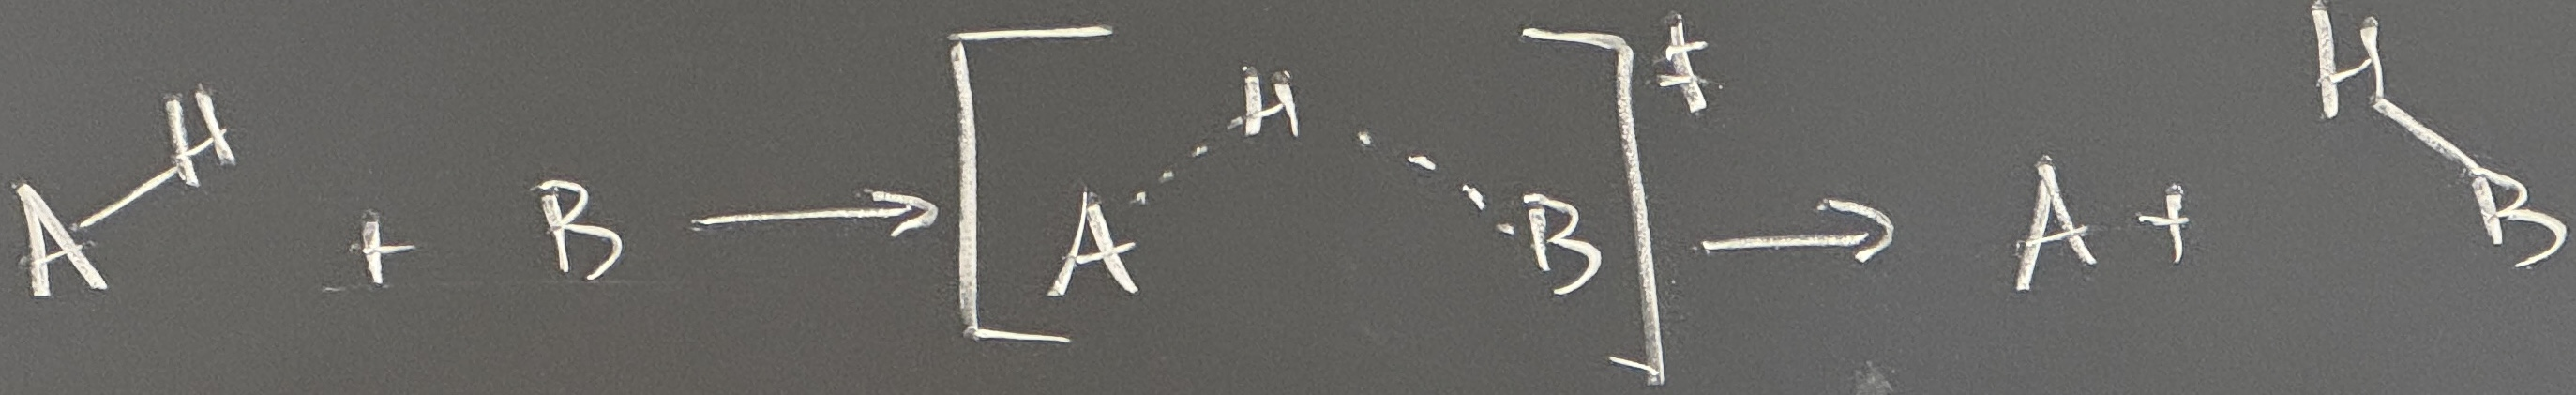
\includegraphics[width=0.45\linewidth]{nonlinearTS.JPG}
        \caption{Nonlinear transition state.}
        \label{fig:nonlinearTS}
    \end{figure}
    \begin{itemize}
        \item We get increasing contributions from the isotopically sensitive bending modes!
        \item This tends to decrease the $\Delta\Delta G^\ddagger$ from the ground state to the transition structure.
        \item This means that $1^\circ$ KIEs can be much smaller.
        \begin{itemize}
            \item Typical range: \numrange{1.5}{3.5}.
        \end{itemize}
        \item Implication: A typical \ce{C-H} stretching mode --- via \ce{R3C-H <=> R_3C***H} --- has $\nu\approx\SI{2900}{\per\centi\meter}$, whereas a typical \ce{C-H} wagging mode --- via \ce{R3C-H <=> R3C-H\,$\updownarrow$} --- has $\nu\approx\SI{1350}{\per\centi\meter}$.
    \end{itemize}
    \item Aside: A reaction that has an anomalous KIE as a result of quantum tunnelling.
    \begin{figure}[h!]
        \centering
        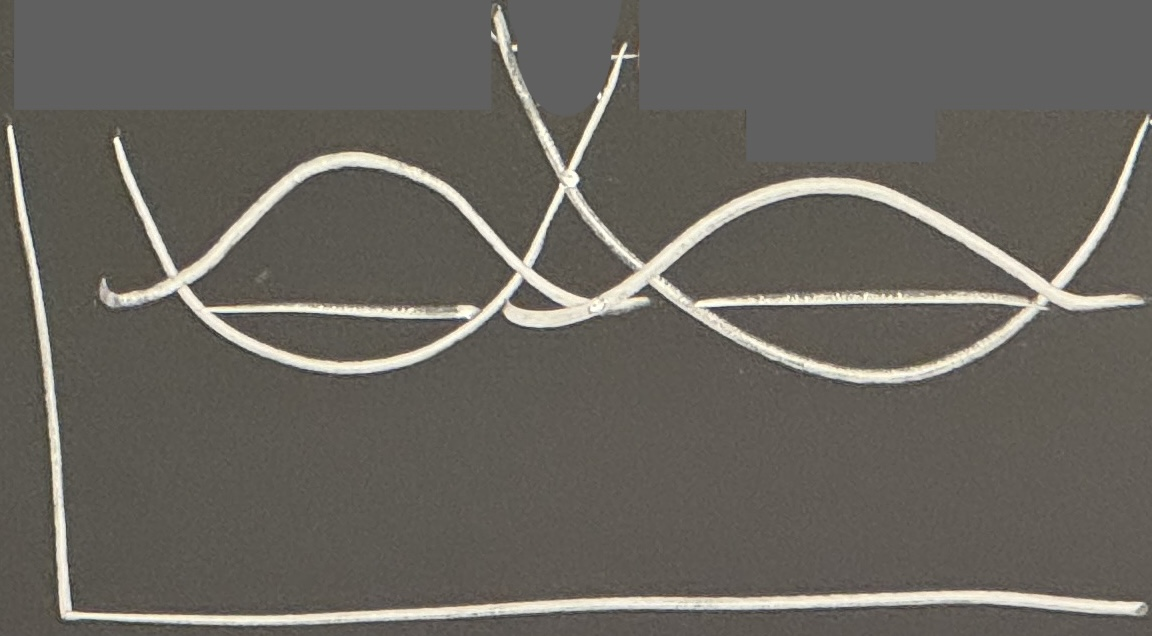
\includegraphics[width=0.3\linewidth]{HATintra.JPG}
        \caption{Intramolecular HAT can proceed through (rather than over) potential barriers.}
        \label{fig:HATintra}
    \end{figure}
    \begin{itemize}
        \item Consider the following intramolecular HAT within the tri-\emph{t}-butylphenyl radical.
        \begin{center}
            \footnotesize
            \schemestart
                \chemfig{*6(-(-{{}^{\emph{t}}Bu})=-(-(<[:-70]Me)(<:[:-30]Me)-[2]-[:150]H/D)=\charge{90=\.}{}-(-{}^{\emph{t}}Bu)=)}
                \arrow
                \chemfig{*6(-(-{{}^{\emph{t}}Bu})=-(-(<[:-70]Me)(<:[:-30]Me)-[2]\charge{90=\.}{})=(-{H/D})-(-{}^{\emph{t}}Bu)=)}
            \schemestop
        \end{center}
        \begin{itemize}
            \item One of the methyl groups is perdeuterated to \ce{CD3}.
        \end{itemize}
        \item Here, $k_{\ce{H}}/k_{\ce{D}}\approx 13000$. Why such a big effect?
        \item The only thing that moves along the reaction coordinate is the proton or deuteron.
        \begin{itemize}
            \item However, it does not have to move \emph{over} the potential barrier here; rather, it can quantum tunnel through it!
            \item This is because per Figure \ref{fig:HATintra}, we get a spread of the vibrational wavefunctions (as we discussed in Figure \ref{fig:quantumOsc}). Thus, the hydrogen can migrate along the reaction coordinate \emph{through} the potential barrier by just decreasing its wave function on one side and increasing it on the other!
            \item Therefore, TST is not applicable here because the first assumption of TST (establishment of a quasi-equilibrium between the SMs and TST) is not met.
        \end{itemize}
        \item Reference: \textcite{bib:HATintra}.
    \end{itemize}
    \item These tunnelling reactions are not all that rare.
    \item Here's some new evidence that a reaction has its product selectivity determined by quantum tunnelling.
    \begin{figure}[H]
        \centering
        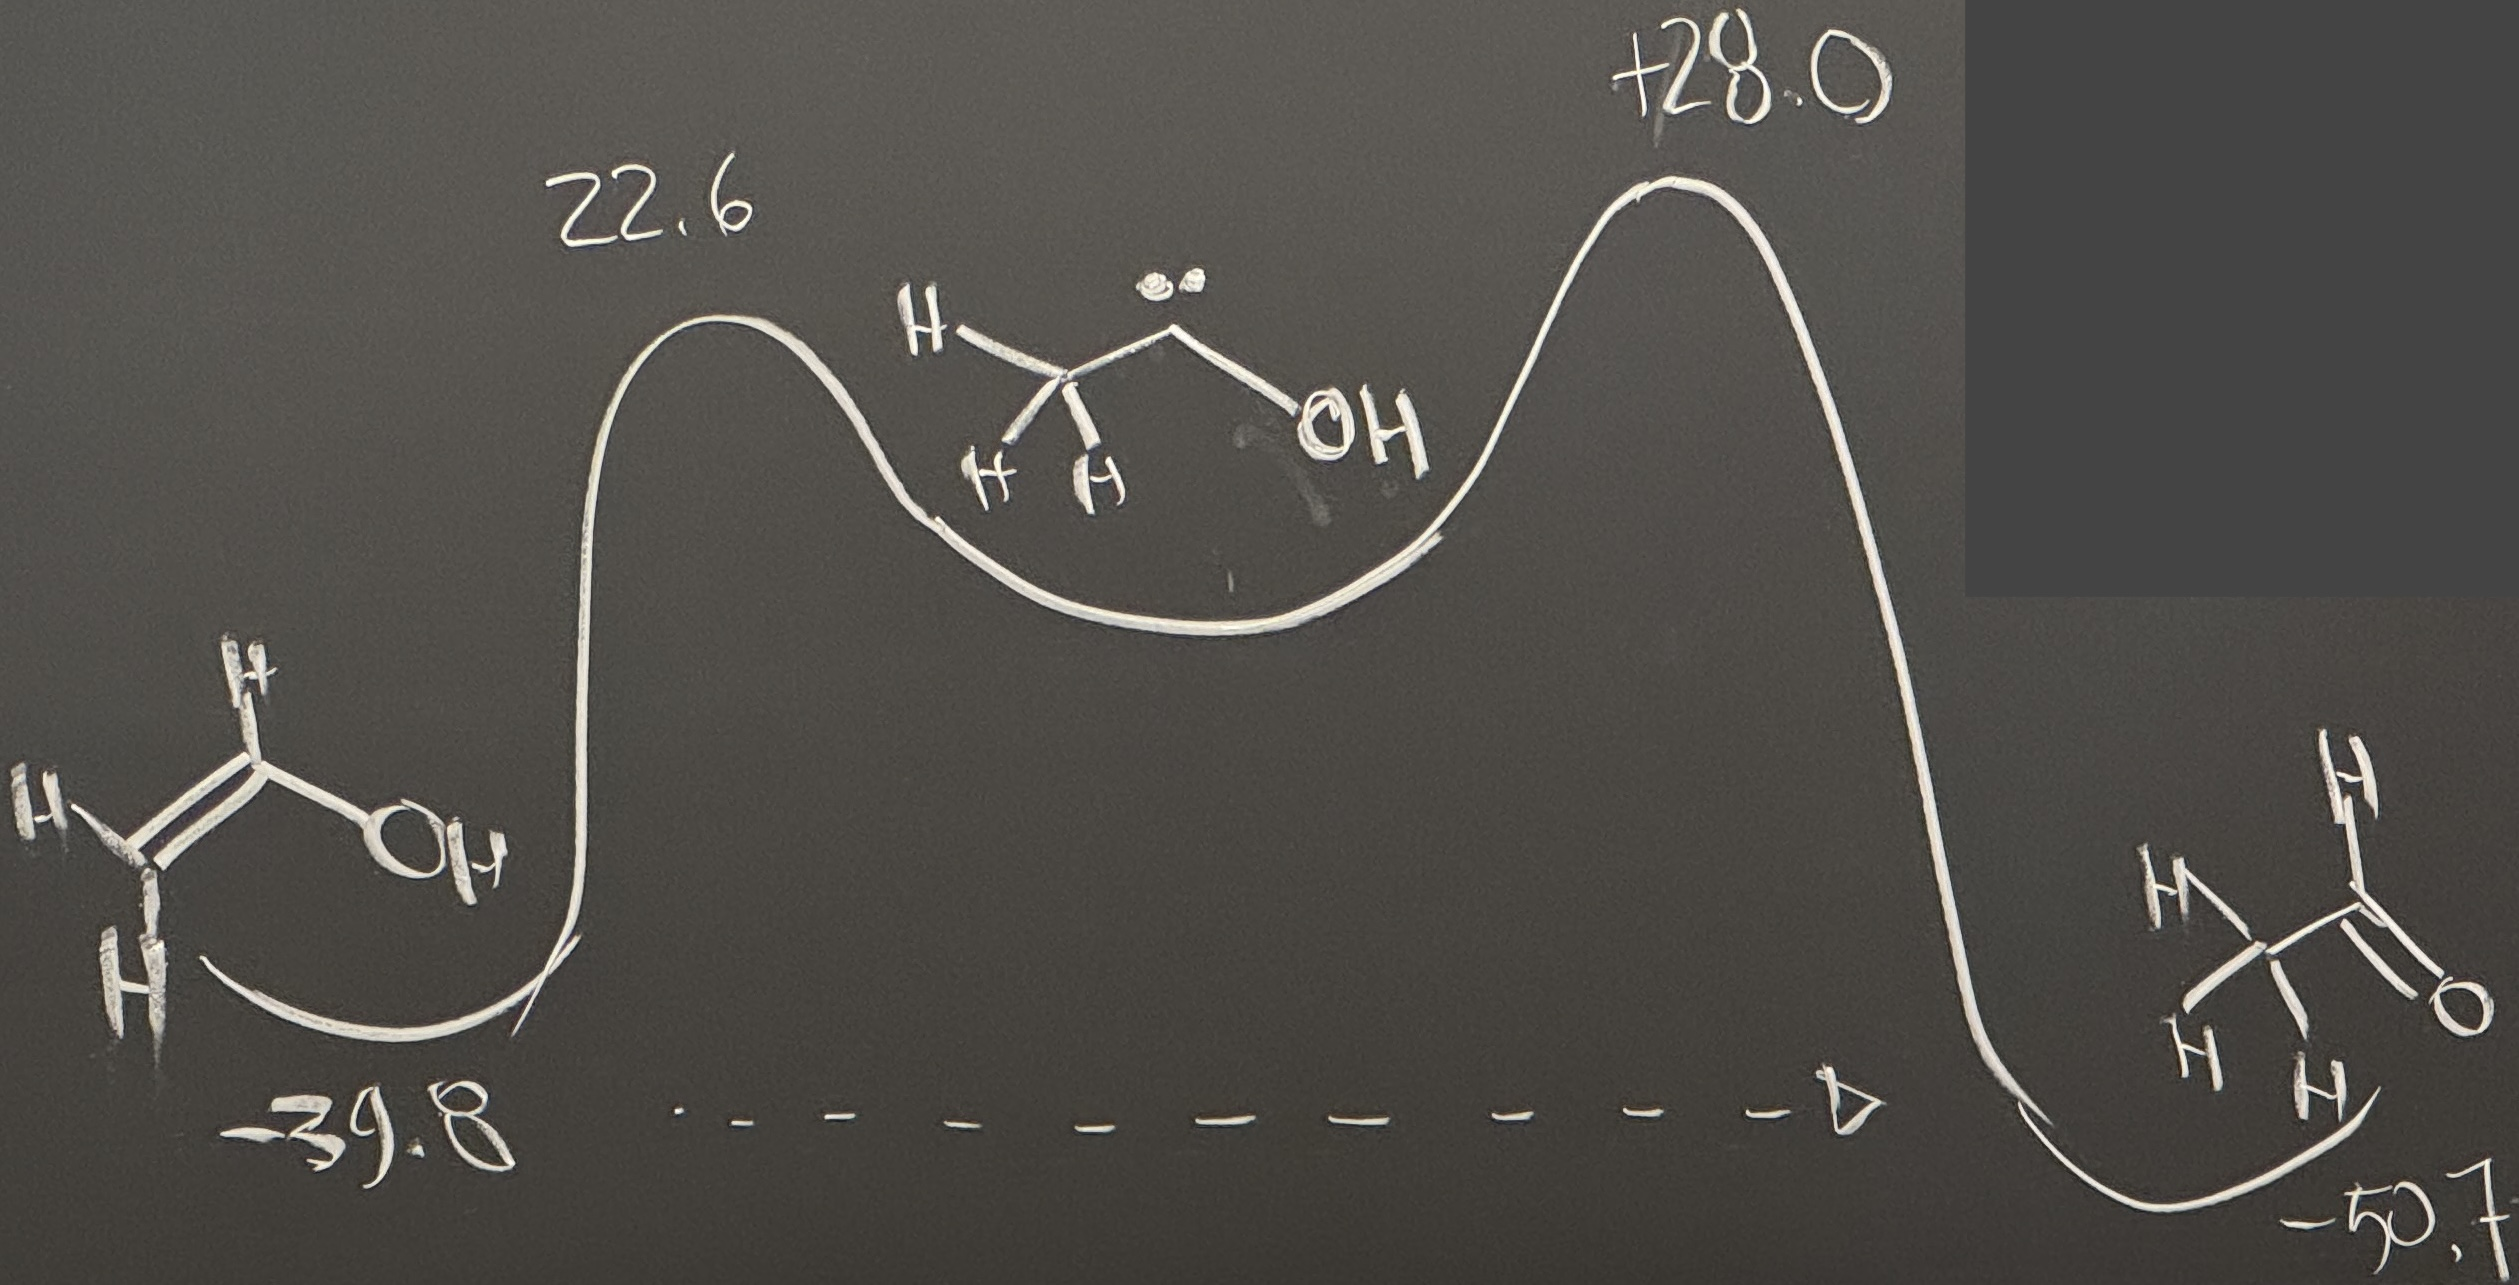
\includegraphics[width=0.5\linewidth]{tunnelSelect.JPG}
        \caption{Quantum tunnelling can influence product selectivity.}
        \label{fig:tunnelSelect}
    \end{figure}
    \begin{itemize}
        \item The reactant is methylhydroxycarbene.
        \begin{itemize}
            \item The adjacent $\pi$-donor makes this carbene a ground-state triplet.
        \end{itemize}
        \item This carbene becomes either acetaldehyde or vinyl alcohol.
        \begin{itemize}
            \item The competing mechanisms are \ce{O-H} and \ce{C-H} migration to the carbene center.
            \item The driving force for formation of vinyl alcohol is $-\kcal{39.8}$.
            \begin{itemize}
                \item The transition state stability for this migration is $+\kcal{22.6}$.
            \end{itemize}
            \item The driving force for formation of acetaldehyde is $-\kcal{50.7}$.
            \begin{itemize}
                \item The transition state stability for this migration is $+\kcal{28}$.
            \end{itemize}
        \end{itemize}
        \item Per transition state theory, \kcal{5} should lead to a \emph{devastating} selectivity for vinyl alcohol.
        \begin{itemize}
            \item Experimentally, however, we observe \emph{exclusive} formation of acetaldehyde.
            \item Note that this reaction is carried out molecule-by-molecule in a matrix at \SI{11}{\kelvin}; i.e., the system is very cold, and every methylhydroxycarbene molecule is isolated from every other and hence allowed to react independently.
        \end{itemize}
        \item Additionally, $t_{1/2}(\ce{H},\ \SI{11}{\kelvin})\approx\SI{1}{\hour}$ and $t_{1/2}(\ce{D},\ \SI{11}{\kelvin})\to\infty$.
        \item Therefore, the mechanism must be quantum tunnelling.
        \item Reference: \textcite{bib:tunnelSelect}.
    \end{itemize}
    \item David: Why would we not get competitive keto-enol tautomerization?
    \begin{itemize}
        \item At \SI{11}{\kelvin}, there's not enough energy for keto-enol tautomerization (even though there is a thermodynamic driving force).
        \item Additionally, keto-enol tautomerization is an intermolecular process, and everything is site isolated in the matrix.
        \item Recall that we don't see uncatalyzed keto-enol tautomerization because it's Woodward-Hoffmann forbidden (see Figure \ref{fig:supraAntarab}). 
        \item This is a good question, because this experiment does rely on zero tautomerization.
    \end{itemize}
    \item Kwanwoo: Temperature dependence of these quantum mechanical effects?
    \begin{itemize}
        \item Quantum tunelling is temperature independent in ways that transition state theory isn't.
    \end{itemize}
    \item A related constellation of isotope effects without primary-ness: Secondary ($2^\circ$) isotope effects.
    \item Let's establish the basics through an example.
    \begin{itemize}
        \item Consider the solvolysis of isopropyl bromide via an S\textsubscript{N}1-like mechanism.
        \begin{center}
            \footnotesize
            \schemestart
                \chemfig{Me-[:30](-[:110]Br)(-[:70]H@{}/D)-[:-30]Me}
                \arrow{->[$k_\text{solv}$]}
                \chemfig{Me-[:30]\charge{[extra sep=4pt]30=$\oplus$}{}(-[2]{H/D})-[:-30]Me}
                \arrow{-->}
            \schemestop
        \end{center}
        \item We assume that $k_\text{solv}$ is the RDS, and everything else is fast.
        \item Recall that $\nu_{\ce{C-H}}\approx\SI{2900}{\per\centi\meter}$.
        \begin{itemize}
            \item In the cation, it's not all that different: $\nu_{\ce{C+-H}}\approx\SI{2800}{\per\centi\meter}$.
        \end{itemize}
        \item The scissoring bend mode --- which brings the proton or deuteron closer to one methyl group or the other --- is approximately \SI{1340}{\per\centi\meter}.
        \begin{itemize}
            \item In the cation, it's also not all that different: \SI{1350}{\per\centi\meter}.
        \end{itemize}
        \item However, the out-of-plane bending mode changes quite a bit: \SI{1340}{\per\centi\meter} to \SI{800}{\per\centi\meter}.
        \item This is the Andy Streitwieser analysis of secondary KIEs: The out of plane bending modes are dominant.
    \end{itemize}
    \item Example: A normal $\alpha$-secondary kinetic isotope effect.
    \begin{itemize}
        \item Consider the solvolysis of a benzyl chloride derivative.
        \begin{center}
            \footnotesize
            \schemestart
                \chemfig{Me-[:30]*6(-=-(-(-[:110]D/H)(-[:70]H@{}/D)-[:-30]Cl)=-=)}
                \arrow{->[\ce{H2O}][\ce{EtOAc}]}
                \chemfig{Me-[:30]*6(-=-(-(-[:110]D/H)(-[:70]H@{}/D)-[:-30]OH)=-=)}
            \schemestop
        \end{center}
        \item Isotopically label the two hydrogens on the active-site carbon.
        \item Through kinetic analysis,\footnote{"We'll get into this in a few lectures" --- is this not just Hammett plots??} we can confirm an S\textsubscript{N}1 mechanism.
        \item Experimentally, we observe that the $\alpha$-$2^\circ$ KIE has $k_{\ce{H}}/k_{\ce{D}}=1.30$.
        \item Let's justify this number.
        \begin{itemize}
            \item The $sp^3$-like starting material goes through an $sp^2$-like transition state.
            \item This means that we're going to a more slack potential, where the out-of-plane bending can happen more freely.
            \item Thus, the \ce{H}/\ce{D} spacing will be tighter in the TS than the ground state, explaining our \emph{normal} KIE (as opposed to an \emph{inverse} KIE).
            \item The number will have a smaller magnitude, however, because it is a secondary effect stabilizing and destabilizing our species, not an atom directly involved in the process.
        \end{itemize}
    \end{itemize}
    \item Example: An inverse $\alpha$-secondary kinetic isotope effect.
    \begin{figure}[h!]
        \centering
        \begin{tikzpicture}[
            every node/.style=black
        ]
            \draw [gry,thick,name path=PESo] (-0.6,3.7)
                to[out=-70,in=180] (0,3.2)
                to[out=0,in=-110] (0.6,3.7)
            ;
            \draw [grx,thick,name path=PES] (-4.5,1.5)
                to[out=-70,in=180,in looseness=0.7] (-3.5,0.8)
                to[out=0,in=180,out looseness=0.7] (0,3.2)
            ;
    
            \path [name path=CH] (-5,1.0) -- ++(3,0);
            \draw [grx,name intersections={of=PES and CH}] (intersection-1) -- (intersection-2);
            \path [name path=CD] (-5,0.9) -- ++(3,0);
            \draw [grx,name intersections={of=PES and CD}] (intersection-1) -- (intersection-2);
    
            \path [name path=C] (-1.5,3.4) -- ++(3,0);
            \draw [gry,name intersections={of=PESo and C}] (intersection-1) -- (intersection-2);
            \path [name path=C] (-1.5,3.6) -- ++(3,0);
            \draw [gry,name intersections={of=PESo and C}] (intersection-1) -- (intersection-2);
        \end{tikzpicture}
        \caption{Inverse $\alpha$-secondary kinetic isotope effect.}
        \label{fig:KIEinvAlph2}
    \end{figure}
    \begin{itemize}
        \item Consider the reaction of anisaldehyde to the corresponding cyanohydrin.
        \begin{center}
            \footnotesize
            \schemestart
                \chemfig{MeO-[:30]*6(-=-(-(=[2]O)-[:-30]H/D)=-=)}
                \arrow{->[\ce{HCN}]}
                \chemfig{Me-[:30]*6(-=-(-(-[2]OH)(<[:-70]CN)<:[:-30]H/D)=-=)}
            \schemestop
        \end{center}
        \item Isotopically label the aldehyde \ce{H}/\ce{D}.
        \item Burgi-Dunitz trajectory to tetrahedral intermediate, which will be thermodynamically uphill.
        \item Here, we have an $sp^2$ SM going to an $sp^3$ TS.
        \item More steric bulk in TS leads to more energetic penalty to wagging, leads to tighter well at the top near the TST.
        \item So we're going from a well with small differences in ZPE to a well with big ZPE differences.
        \item This penalizes access to the TST with hydrogen, giving us an inverse KIE of 0.7.
    \end{itemize}
    \pagebreak
    \item We now move onto $\beta$-secondary KIEs.
    \item Example: Labeling $\beta$ to the "active site."
    \begin{itemize}
        \item Consider the base-mediated elimination (E\textsubscript{2} dehydrohalogenation) of 1-propylbromide.
        \begin{center}
            \footnotesize
            \schemestart
                \chemfig{Me-[:30](-[:110]D/H)(-[:70]H@{}/D)-[:-30]-[:30]Br}
                \arrow{->[\ce{NaOEt}][\ce{EtOH}]}[,1.2]
                \chemfig{Me-[:30](-[2]{H/D})=_[:-30]}
            \schemestop
        \end{center}
        \item We label $\beta$ to the bromide.
        \item Displacement of the bromide is concommittant with \ce{C-H} cleavage at the $\beta$-position, so we should see a large KIE.
        \begin{itemize}
            \item Indeed we do: $k_{\ce{H}}/k_{\ce{D}}=6.7$.
        \end{itemize}
        \item So frankly, this is a $1^\circ$ KIE.
    \end{itemize}
    \item Example: A real normal $\beta$-secondary kinetic isotope effect.
    \begin{itemize}
        \item Consider the E\textsubscript{1} dehydrohalogenation of 1-propylbromide.
        \begin{center}
            \footnotesize
            \schemestart
                \chemfig{Me-[:30](-[:110]D/H)(-[:70]H@{}/D)-[:-30]-[:30]Br}
                \arrow{->[\ce{H2O}][$\Delta$]}[,1.2]
                \chemfig{Me-[:30](-[2]{H/D})=_[:-30]}
            \schemestop
        \end{center}
        \item Here, rate-limiting loss of \ce{Br} gives a cation intermediate.
        \begin{itemize}
            \item There is no change in hybridization at the $\beta$-position.
            \item However, we do have a donor-acceptor interaction. Indeed, there is symmetry-allowed $\sigma_{\ce{C-H/D}}\to p_{\ce{C}}$ mixing.
            \item This depopulates the $\beta$-bonding orbital.
            \item Depopulating this orbital leads to weaker bonds, smaller force constants, and a more slack potential in the transition state.
            \item So if we're going to a more slack potential, we get normal KIEs.
        \end{itemize}
        \item Indeed, $k_{\ce{H}}/k_{\ce{D}}=1.4$.
        \begin{itemize}
            \item This kinetic isotope effect is greater than 1 for all the reasons we've talked about.
            \item However, the \ce{C-H/D} bond is not being cleaved in the transition state, so the magnitude is still relatively small.
        \end{itemize}
    \end{itemize}
    \item Secondary KIEs are usually smaller because they're not at the reactive center.
    \begin{itemize}
        \item Secondary KIEs will rarely be bigger than 1.5 or smaller than 0.7.
    \end{itemize}
    \item All of this is a prelude to what he actually want's to talk about: This lecture's content, which will mostly become next lecture's content.
    \item Experimental determination of KIEs.
    \begin{itemize}
        \item Nicely summarized in a paper 10-12 years ago by Eric Simmons (now at BMS) and John Hartwig.
        \item Read this before next time in order to dialogue about what's going on!!
        \item Reference: \textcite{bib:KIEexpt}.
    \end{itemize}
    \pagebreak
    \item First and least interesting method: Independent absolute rate measurement.
    \begin{figure}[h!]
        \centering
        \footnotesize
        \begin{subfigure}[b]{0.4\linewidth}
            \centering
            \schemestart
                \chemfig{*6(-=-(-H)=-=)}
                \arrow{->[$k_{\ce{H},\text{expt}}$]}[,1.2]
                \chemfig{*6(-=-(-FG)=-=)}
            \schemestop
            \caption{Undeuterated.}
            \label{fig:indepAbsRatea}
        \end{subfigure}
        \begin{subfigure}[b]{0.4\linewidth}
            \centering
            \schemestart
                \chemfig{*6(-=-(-D)=-=)}
                \arrow{->[$k_{\ce{D},\text{expt}}$]}[,1.2]
                \chemfig{*6(-=-(-FG)=-=)}
            \schemestop
            \caption{Deuterated.}
            \label{fig:indepAbsRateb}
        \end{subfigure}
        \caption{Independent absolute rate measurement of kinetic isotope effects.}
        \label{fig:indepAbsRate}
    \end{figure}
    \begin{itemize}
        \item Consider the functionaliztion of an arene, one sample deuterated and the other not.
        \item First measure $k_{\ce{H}}$, and then measure $k_{\ce{D}}$. Take the ratio of these independently measured rate constants as your KIE.
        \item This works and people do this, but a few things make it difficult.
        \begin{enumerate}
            \item Absolute (as opposed to relative) determinations of rate constants are prone to error.
            \begin{itemize}
                \item You have error associated with the determination of each of each.
                \item Your KIE is only as good as the accuracy of each independent KIE, so we get propagation of error.
            \end{itemize}
            \item Despite our best attempts, there will be small variations in the way these reactions are executed (e.g., different concentrations, different temperatures, etc.), contributing to our error.
            \item Only reports on reactions when RDS is isotope-sensitive.
            \begin{itemize}
                \item Only really useful if the bond with the isotope is sensitive to cleavage in the RDS.
                \item So good when the initial transition state structure is rate-determining and isotopically sensitive.
                \item What if the first step is rate-determining, but not isotopically sensitive? In this case, our rate analysis is useless because everything else is post-rate limiting.
            \end{itemize}
        \end{enumerate}
        \item So these are difficult experimentally and "blind" to post-rate limiting steps.
    \end{itemize}
    \item Next time: Stuff that allows us to see post-rate limiting transformations.
\end{itemize}




\end{document}